\documentclass[10pt,twocolumn]{article}

% Packages
\usepackage[utf8]{inputenc}
\usepackage{amsmath,amssymb,amsfonts}
\usepackage{algorithmic}
\usepackage{algorithm}
\usepackage{graphicx}
\usepackage{textcomp}
\usepackage{booktabs}
\usepackage{multirow}
\usepackage{hyperref}
\usepackage{xcolor}
\usepackage{subcaption}
\usepackage[margin=1in]{geometry}
\usepackage{microtype}
\usepackage{amsthm}
\newtheorem{theorem}{Theorem}
\newtheorem{proposition}[theorem]{Proposition}
\graphicspath{{figures/}{cifar100_figures/}}

% Custom commands
\newcommand{\method}{LAFTJU}
\newcommand{\methodfull}{Layer-wise Adaptive Kronecker-Factored Trajectory Unified Optimizer}
\newcommand{\R}{\mathbb{R}}
\newcommand{\E}{\mathbb{E}}

\title{\method{}: \methodfull{}}

\author{
  Anonymous
}

\date{}

\begin{document}

\maketitle

% ============================================================
% Abstract
% ============================================================
\begin{abstract}
We propose \method{} (\methodfull{}), a novel optimization algorithm that unifies curvature-aware trajectory optimization with adaptive gradient methods through a homotopy-based blending mechanism. \method{} employs Kronecker-factored preconditioning for efficient second-order curvature approximation, a tanh-based homotopy scheduler for smooth transition between optimization paths, and layer-wise adaptive coupling. On CIFAR-10 with ResNet-18, \method{} achieves a best test accuracy of \textbf{95.82\%}, surpassing Adam (93.99\%) and AdamW (94.55\%). We further introduce \method{}-NS, a near-first-order variant using Newton-Schulz orthogonalization that achieves \textbf{95.27\%} test accuracy with only $2.1\times$ AdamW overhead and 244\,MB memory---25\% faster and 30\% less memory than full \method{}. On CIFAR-100 with fair baseline tuning, \method{}-NS achieves \textbf{75.43\%$\pm$0.30\%} (5 seeds), outperforming Adam (74.09\%) and AdamW (74.68\%). On PTB language modeling with AWD-LSTM, \method{}-NS achieves the best test perplexity across all configurations: \textbf{82.30$\pm$0.26} (1-layer), \textbf{65.29$\pm$0.12} (2-layer), and \textbf{61.83$\pm$0.15} (3-layer), consistently outperforming Adam (82.73, 65.64, 61.88) and significantly surpassing AdamW (88.34, 72.03, 68.78). On BERT-base fine-tuning across all 7 GLUE tasks, \method{}-NS \textbf{outperforms AdamW on every task}, achieving an average improvement of +0.32\% with the largest gains on CoLA (+1.05) and SST-2 (+0.46). On Transformer-XL (151.1M) language modeling on WikiText-103, \method{}-NS achieves a statistically significant improvement over AdamW at matched learning rate (\textbf{42.08$\pm$0.10} vs.\ 42.36$\pm$0.12 test PPL, $p$=0.005), while both optimizers benefit equally from higher learning rates (36.15 vs.\ 36.01 at lr=5e-4). On GPT-2 Small (124M) pretraining, \method{}-NS matches AdamW (19.35 vs.\ 19.37 PPL) with only 1.01$\times$ overhead, while at GPT-2 Medium scale (354M) the advantage persists. We provide rigorous convergence analysis grounded in dynamical systems theory: we prove complete stability via a time-varying Lyapunov function, establish equivalence between local optimal solutions and stable equilibrium points, derive super-exponential approximation bounds for Newton-Schulz orthogonalization ($O(\rho^{5^K})$), and prove $O(1/\sqrt{T})$ convergence rate for the stochastic discrete-time setting. These results demonstrate that NS orthogonalization benefits diverse architectures---CNNs, RNNs, and Transformers---when properly configured.
\end{abstract}

% ============================================================
% 1. Introduction
% ============================================================
\section{Introduction}

Deep neural network optimization remains a central challenge in machine learning. First-order methods such as Adam~\cite{adam} dominate practice, while second-order methods offer faster convergence but at prohibitive computational cost. Recent work on AdamW~\cite{adamw} and various hybrid approaches attempts to bridge this gap.

We identify several limitations in existing approaches: (1) pure first-order methods ignore curvature information, leading to slow convergence in ill-conditioned landscapes; (2) second-order methods (K-FAC, natural gradient) are too expensive for practical use; (3) existing hybrid methods lack principled mechanisms for blending different optimization strategies.

To address these challenges, we propose \method{}, which makes the following contributions:
\begin{itemize}
    \item A \textbf{dual-path optimization framework} that combines curvature-aware trajectory optimization (TJU path) with adaptive gradient methods (AdamW path) through a principled homotopy blending mechanism.
    \item An efficient \textbf{Kronecker-factored preconditioning} (KF-PTC) scheme that provides approximate second-order information for convolutional and linear layers at minimal overhead. A diagonal variant (\method{}-Lite) reduces memory to $O(m+n)$ per layer and eliminates matrix inversion, achieving $\sim\!1.87\times$ AdamW overhead.
    \item A \textbf{Newton-Schulz orthogonalization} variant (\method{}-NS) that replaces all Kronecker-factor matrices with a quintic iterative polar decomposition applied directly to the gradient EMA matrix. With interval-based amortization (every 10 steps) and bfloat16 acceleration, \method{}-NS achieves \textbf{95.27\%} on CIFAR-10 at only $1.92\times$ AdamW overhead and 244\,MB memory---25\% faster and 30\% less memory than full \method{} while still surpassing all first-order baselines.
    \item A \textbf{tanh-based homotopy scheduler} that smoothly transitions from exploration (TJU-dominated) to exploitation (AdamW-dominated) during training.
    \item A \textbf{rigorous convergence theory} grounded in dynamical systems analysis: we prove complete stability via a time-varying Lyapunov function, establish local-optimal-solution/stable-equilibrium equivalence, derive super-exponential NS approximation bounds, and prove $O(1/\sqrt{T})$ stochastic convergence matching AdamW.
    \item Comprehensive experimental evaluation on CIFAR-10, CIFAR-100, PTB language modeling, BERT GLUE fine-tuning, GPT-2 pretraining (124M and 354M), and Transformer-XL language modeling, including comparisons with modern optimizers (Lion, Adan), demonstrating competitive or superior performance across vision, language modeling, and language model pretraining tasks with negligible overhead (1.01$\times$ AdamW at Transformer scale).
\end{itemize}

% ============================================================
% 2. Related Work
% ============================================================
\section{Related Work}

\textbf{First-order methods.} Adam~\cite{adam} and its weight-decay-corrected variant AdamW~\cite{adamw} are widely used for their adaptive learning rate properties. Lion~\cite{lion}, discovered via program search, uses only sign operations and a single momentum buffer, achieving competitive performance with lower memory. Adan~\cite{adan} introduces a Nesterov-style triple-momentum scheme that achieves strong results across vision and language tasks.

\textbf{Second-order methods.} K-FAC~\cite{kfac} approximates the Fisher information matrix using Kronecker-factored representations, reducing the cost from $O(n^3)$ to $O(n^{3/2})$ per layer. Shampoo~\cite{shampoo} extends this idea with online preconditioning.

\textbf{Near-first-order second-order methods.} Recent work attempts to recover second-order benefits at first-order cost. SOAP~\cite{soap} observes that Shampoo with a $1/2$-power preconditioner is equivalent to Adam in the eigenbasis of the input/output covariance matrices; by running Adam's second-moment update every step in the \emph{current} eigenbasis and updating the eigenbasis infrequently, SOAP achieves a 35\% wall-clock reduction over AdamW on transformer training. Muon~\cite{muon} takes a different route: it applies a Newton-Schulz (NS) iteration~\cite{kosson} to orthogonalize the gradient update matrix, computing an approximate polar factor $U \approx G(G^\top G)^{-1/2}$ in $O(P)$ per step with 5 matrix-multiply iterations and no stored curvature matrices. Muon set CIFAR-10 speedrunning records and reduced required training iterations by $\sim\!40\%$ vs.\ AdamW. Our \method{}-NS directly adapts this NS orthogonalization into the TJU homotopy path.

\textbf{Sharpness-aware methods.} SAM~\cite{sam} minimizes both the loss value and loss sharpness, leading to flatter minima with better generalization. ASAM extends SAM with adaptive perturbation radii.

\textbf{Hybrid approaches.} Several works combine different optimization strategies, but few provide principled mechanisms for transitioning between them. Our homotopy-based approach offers a smooth, controllable blending schedule grounded in continuation methods from numerical analysis.

% ============================================================
% 3. Method
% ============================================================
\section{Method}

\subsection{Overview}

\method{} maintains two parallel optimization paths and blends their updates through a homotopy parameter $s(t)$. At each step $t$, the parameter update is:
\begin{equation}
\Delta \theta_t = -(1-s_t) \cdot \alpha_{\text{tju}} \cdot \mathbf{u}_t^{\text{TJU}} - s_t \cdot \alpha_{\text{a}} \cdot (\mathbf{u}_t^{\text{AdamW}} + \lambda \theta_t)
\label{eq:blending}
\end{equation}
where $\mathbf{u}_t^{\text{TJU}}$ is the curvature-preconditioned update, $\mathbf{u}_t^{\text{AdamW}}$ is the standard AdamW update, $\alpha_{\text{tju}}$ and $\alpha_{\text{a}}$ are respective learning rates, $\lambda$ is the weight decay coefficient, and $s_t \in [0,1]$ is the homotopy blending parameter.

\subsection{TJU Path: Curvature-Aware Trajectory Optimization}

The TJU (Trajectory Unified) path maintains exponential moving averages of the gradient and an approximate diagonal Hessian:
\begin{align}
\mathbf{m}_t &= \beta_1 \mathbf{m}_{t-1} + (1-\beta_1) \nabla \mathcal{L}_t \\
\hat{\mathbf{m}}_t &= \mathbf{m}_t / (1 - \beta_1^t)
\end{align}
where L2 weight decay is folded into the gradient: $\nabla \mathcal{L}_t \leftarrow \nabla \mathcal{L}_t + \lambda \theta_t$.

For parameters with Kronecker-factored preconditioning available (Conv2d and Linear layers), the update is:
\begin{equation}
\mathbf{u}_t^{\text{TJU}} = \mathbf{P}_t^{-1} \hat{\mathbf{m}}_t
\end{equation}
where $\mathbf{P}_t$ is the Kronecker-factored preconditioner (detailed in Section~\ref{sec:kfptc}).

For 1D parameters (batch normalization, biases), a diagonal Hessian approximation is used as fallback:
\begin{equation}
\mathbf{u}_t^{\text{TJU}} = \hat{\mathbf{m}}_t / |\mathbf{H}_t^{\text{diag}}|
\end{equation}

\subsection{AdamW Path}

The AdamW path follows the standard AdamW formulation:
\begin{align}
\mathbf{m}_t^a &= \beta_1 \mathbf{m}_{t-1}^a + (1-\beta_1) \nabla \mathcal{L}_t \\
\mathbf{v}_t^a &= \beta_2 \mathbf{v}_{t-1}^a + (1-\beta_2) (\nabla \mathcal{L}_t)^2 \\
\mathbf{u}_t^{\text{AdamW}} &= \frac{\hat{\mathbf{m}}_t^a}{\sqrt{\hat{\mathbf{v}}_t^a} + \epsilon}
\end{align}
with bias-corrected estimates $\hat{\mathbf{m}}_t^a$ and $\hat{\mathbf{v}}_t^a$.

\subsection{Kronecker-Factored Preconditioning (KF-PTC)}
\label{sec:kfptc}

For a layer with weight matrix $W \in \R^{m \times n}$, the Fisher information matrix $F$ can be approximated as:
\begin{equation}
F \approx A \otimes G
\end{equation}
where $A = \E[\mathbf{a}\mathbf{a}^\top] \in \R^{n \times n}$ is the input activation covariance and $G = \E[\mathbf{g}\mathbf{g}^\top] \in \R^{m \times m}$ is the output gradient covariance. The preconditioned gradient is then:
\begin{equation}
\text{vec}(\tilde{\nabla}_W) = (A + \delta I)^{-1} \text{vec}(\nabla_W) (G + \delta I)^{-1}
\end{equation}
where $\delta$ is a damping factor for numerical stability.

\method{} registers forward and backward hooks to collect activation and gradient statistics, updating the Kronecker factors every $T_{\text{kf}}$ steps using exponential moving averages:
\begin{align}
A_t &= \rho A_{t-1} + (1-\rho) \mathbf{a}_t \mathbf{a}_t^\top \\
G_t &= \rho G_{t-1} + (1-\rho) \mathbf{g}_t \mathbf{g}_t^\top
\end{align}
with EMA coefficient $\rho = 0.95$ and update interval $T_{\text{kf}} = 20$.

For convolutional layers, input activations are spatially averaged (mean over $H \times W$) to obtain a compact $(B, C_{\text{in}})$ representation before computing covariance factors, avoiding the large temporary tensors produced by full \texttt{im2col} unfolding.

\textbf{Diagonal KF variant (\method{}-Lite).} The full KF scheme stores $A \in \R^{n\times n}$ and $G \in \R^{m\times m}$ per layer, incurring $O(C^2)$ memory and $O(C^3)$ inversion cost. We propose a diagonal approximation that retains only the per-channel variances:
\begin{align}
\mathbf{a}_j &= \E[\bar{a}_j^2], \quad j = 1,\ldots,n \\
\mathbf{g}_i &= \E[\bar{g}_i^2], \quad i = 1,\ldots,m
\end{align}
The preconditioned gradient element $(i,j)$ is then:
\begin{equation}
\tilde{\nabla}_{ij} = \frac{\nabla_{ij}}{\sqrt{(\mathbf{g}_i + \delta)(\mathbf{a}_j + \delta)}}
\label{eq:diagkf}
\end{equation}
This reduces per-layer memory from $O(m^2 + n^2)$ to $O(m+n)$, eliminates matrix inversion entirely, and reduces hook computation from $O(C^2)$ to $O(C)$ per step. The sqrt normalization in Eq.~\eqref{eq:diagkf} matches Adam's variance-normalization convention and stabilizes early training. \method{}-Lite uses this diagonal KF throughout, achieving $\sim\!1.87\times$ AdamW overhead vs $\sim\!3\times$ for full KF.

\subsection{Newton-Schulz Orthogonalization (\method{}-NS)}
\label{sec:ns}

Although \method{}-Lite achieves $O(P)$ memory and complexity, it retains a hook-based data-collection step and stores per-channel variance vectors. Inspired by Muon~\cite{muon} and the polar decomposition approach of Kosson et al.~\cite{kosson}, we propose \method{}-NS, which eliminates \emph{all} Kronecker-factor storage and hooks.

\textbf{Motivation.} For a weight matrix $W \in \R^{m \times n}$, the optimal preconditioned update direction under an isotropic curvature assumption is the \emph{polar factor}:
\begin{equation}
U = (G^\top G)^{-1/2} G, \quad G = \hat{\mathbf{m}}_t \in \R^{m \times n}
\label{eq:polar}
\end{equation}
$U$ orthogonalizes the gradient so that all singular directions receive equal step size, removing ill-conditioning while preserving directionality. This is precisely what Shampoo computes with its $1/2$-power preconditioner~\cite{soap}.

\textbf{Newton-Schulz iteration.} Computing the polar factor via SVD costs $O(\min(m,n) \cdot mn)$. Instead, \method{}-NS uses a degree-5 Chebyshev-Newton-Schulz iteration~\cite{kosson,muon} that avoids SVD entirely:
\begin{align}
X_0 &= G / \|G\|_F \notag \\
X_{k+1} &= \tfrac{15}{8} X_k - \tfrac{35}{24} X_k (X_k^\top X_k) \notag \\
&\quad + \tfrac{21}{40} X_k (X_k^\top X_k)^2 - \tfrac{5}{112} X_k (X_k^\top X_k)^3
\label{eq:ns}
\end{align}
After $K=5$ iterations, $X_K \approx U$ up to numerical precision in float32. Each iteration requires 3--4 matrix multiplications of the form $X_k X_k^\top X_k$ (shape $m \times n$), totaling $O(K \cdot mn) = O(P)$ flops per parameter. No matrices larger than the weight tensor itself are ever formed.

\textbf{Rescaling.} Since $\|U\|_F \approx \sqrt{\min(m,n)}$ while $\|\hat{m}_t\|_F$ varies with gradient magnitude, we rescale the orthogonalized update to match the gradient norm:
\begin{equation}
\mathbf{u}_t^{\text{NS}} = X_K \cdot \frac{\|\hat{\mathbf{m}}_t\|_F}{\|X_K\|_F + \epsilon}
\label{eq:ns_rescale}
\end{equation}
This ensures the NS update direction contributes at the same magnitude as the AdamW path in the homotopy blend.

\textbf{Algorithm.} \method{}-NS uses the same dual-path homotopy as \method{} (Eq.~\eqref{eq:blending}), but replaces the KF preconditioned update with the NS-orthogonalized update:
\begin{equation}
\mathbf{u}_t^{\text{TJU}} = \mathbf{u}_t^{\text{NS}} \quad \text{(for 2-D weight tensors)}
\end{equation}
For 1-D parameters (biases, batch normalization), \method{}-NS falls back to the AdamW update $\mathbf{u}_t^{\text{AdamW}}$. The shared Adam moment buffers ($\mathbf{m}_1$, $\mathbf{m}_2$) are reused for both paths.

\textbf{Interval-based amortization.} Computing NS orthogonalization every step is unnecessary since the gradient EMA changes slowly. \method{}-NS recomputes the NS direction every $T_{\text{ns}}$ steps and caches the result; on intermediate steps, the cached direction is rescaled to match the current gradient magnitude:
\begin{equation}
\mathbf{u}_t^{\text{NS}} = \mathbf{u}_{\lfloor t/T_{\text{ns}} \rfloor \cdot T_{\text{ns}}}^{\text{NS}} \cdot \frac{\|\hat{\mathbf{m}}_t\|_F}{\|\mathbf{u}_{\text{cached}}\|_F + \epsilon}
\end{equation}
This amortizes the 5-GEMM cost over $T_{\text{ns}}$ steps. Combined with bfloat16 computation for the NS iterations, the measured overhead is $1.92\times$ AdamW (6.90\,ms vs.\ 3.69\,ms per step on ResNet-18/CIFAR-10).

\textbf{Gradient centralization.} For all $\geq$2D weight tensors, \method{}-NS subtracts the per-output-channel gradient mean before moment updates:
\begin{equation}
\nabla_{ij} \leftarrow \nabla_{ij} - \frac{1}{n}\sum_{k=1}^{n} \nabla_{ik}
\end{equation}
This constrains updates to the zero-mean subspace, improving generalization at negligible cost~\cite{gc}.

\textbf{Complexity summary.} \method{}-NS requires exactly $2P$ memory (Adam moments, same as AdamW), zero hook registrations, zero stored factor matrices, and $O(KP) \approx O(P)$ arithmetic per step. With interval-based amortization (recomputing NS every $T_{\text{ns}}=10$ steps and caching the orthogonalized direction), the effective per-step cost is further reduced:

\begin{table}[ht]
\centering
\small
\caption{Memory and per-step complexity comparison. $P$: total parameters, $L$: layers, $C$: average width, $K$: NS iterations (5), $T_{\text{ns}}$: NS interval (10).}
\label{tab:complexity}
\resizebox{\columnwidth}{!}{%
\begin{tabular}{@{}llll@{}}
\toprule
\textbf{Optimizer} & \textbf{Memory} & \textbf{Per-step cost} & \textbf{Measured} \\
\midrule
AdamW         & $2P$                 & $O(P)$ & 3.69\,ms \\
\method{}$^\dagger$ & $5P + 4LC^2$    & $O(P + LC^3/T_{\text{kf}})$ & 10.56\,ms \\
\textbf{\method{}-NS} & $\mathbf{2P}$ & $\mathbf{O(KP/T_{\text{ns}})}$ & \textbf{6.90\,ms} \\
\bottomrule
\end{tabular}%
}
\end{table}

\subsection{Homotopy Scheduler}

The homotopy parameter $s_t$ controls the blend between TJU and AdamW paths:
\begin{equation}
s_t = \tanh\!\left(\frac{t}{T} \cdot \eta\right)
\label{eq:homotopy}
\end{equation}
where $T$ is the total number of training steps and $\eta$ is the homotopy speed. At the beginning of training ($t \ll T$), $s_t \approx 0$ and the TJU path dominates, leveraging curvature information for rapid initial progress. As training progresses, $s_t \to 1$ and the AdamW path takes over for fine-grained convergence.

The homotopy speed $\eta$ controls how quickly the transition occurs. Our experiments reveal that $\eta$ must be carefully tuned in relation to the total training epochs (see Section~\ref{sec:ablation}).

\subsection{Learning Rate Schedule}

\method{} uses a dual-track cosine annealing schedule:
\begin{align}
\alpha_{\text{tju}}(t) &= \alpha_{\text{tju}}^{\min} + \frac{1}{2}(\alpha_{\text{tju}}^0 - \alpha_{\text{tju}}^{\min})(1 + \cos(\pi t / T)) \\
\alpha_{\text{a}}(t) &= \alpha_{\text{a}}^{\min} + \frac{1}{2}(\alpha_{\text{a}}^0 - \alpha_{\text{a}}^{\min})(1 + \cos(\pi t / T))
\end{align}
with a linear warmup phase during the first $W$ steps where both learning rates are scaled by $t/W$.

\subsection{Theoretical Analysis}
\label{sec:theory}

We establish convergence guarantees for \method{} by analyzing it as a nonlinear dynamical system, extending the HTJU framework~\cite{htju} to accommodate (i) the tanh-based homotopy schedule, (ii) Kronecker-factored and Newton-Schulz preconditioning, and (iii) the discrete-time stochastic setting.

\subsubsection{LAFTJU as a Nonlinear Dynamical System}

Consider the non-convex optimization problem $\min_w h(w) = \frac{1}{N}\sum_{i=1}^N \ell(f(w,z_i), y_i)$. Define the stacked loss vector $H(w) = [h(w,z_1); \ldots; h(w,z_N)]$. The \method{} parameter dynamics (Eq.~\eqref{eq:blending}) correspond to the continuous-time ODE:
\begin{equation}
\dot{w} = -(1-s(t)) \cdot P_t^{-1} \nabla H(w)^\top H(w) - s(t) \cdot \nabla H(w),
\label{eq:ode}
\end{equation}
where $P_t$ denotes the preconditioner (Kronecker-factored, diagonal, or Newton-Schulz), and $s(t) = \tanh(t \eta / T)$ is the homotopy parameter. The first term is the curvature-preconditioned TJU path; the second is the first-order AdamW path. Since $\tanh$ is $C^\infty$ and monotonically increasing on $[0,\infty)$, the vector field in Eq.~\eqref{eq:ode} is smooth in both $w$ and $t$.

\subsubsection{Stability Region and Equilibrium Characterization}

An equilibrium point $w_e$ satisfies $\dot{w}|_{w=w_e} = 0$, which requires $\nabla H(w_e)^\top H(w_e) = 0$ (first-order stationarity). We call $w_e$ a \emph{stable equilibrium point} (SEP) if all eigenvalues of the Jacobian $J(w_e) = \nabla^2_{ww} H(w_e)$ have strictly negative real parts. The \emph{stability region} $A(w_e)$ is the set of initial conditions whose trajectories converge to $w_e$.

We require the following assumptions, standard in dynamical systems theory~\cite{htju}:
\begin{itemize}
\item[\textbf{A1}] (Hyperbolicity) All equilibrium points on the stability boundary $\partial A(w_e)$ are hyperbolic.
\item[\textbf{A2}] (Transversality) The stable and unstable manifolds of boundary equilibria intersect transversally.
\item[\textbf{A3}] (Boundary approach) Every trajectory on $\partial A(w_e)$ converges to a boundary equilibrium as $t \to \infty$.
\end{itemize}

\begin{theorem}[Stability Boundary Characterization]
\label{thm:boundary}
Consider the \method{} dynamics~\eqref{eq:ode} satisfying A1--A3. Let $\{w_i^e\}_{i \geq 1}$ denote the equilibrium points on $\partial A(w_s)$ of a SEP $w_s$. Then the stability boundary is:
\begin{equation}
\partial A(w_s) = \bigcup_{i \geq 1} W^s(w_i^e),
\end{equation}
where $W^s(w_i^e)$ is the stable manifold of the boundary equilibrium $w_i^e$.
\end{theorem}

\begin{proof}[Proof sketch]
The proof follows the structure of~\cite{htju}, Theorem~1. Forward invariance of $\partial A(w_s)$ and the stable manifold theorem give $\partial A(w_s) \supseteq \bigcup_i W^s(w_i^e)$. Reverse inclusion follows from A3: any $w \in \partial A(w_s)$ must lie on some $W^s(w_i^e)$. The tanh homotopy does not alter the equilibrium structure since $s(t)$ is a scalar multiplier that preserves the zero set of $\nabla H(w)^\top H(w)$. Full details are in Appendix~\ref{app:proofs}.
\end{proof}

\subsubsection{Complete Stability and Trajectory Convergence}

\begin{theorem}[Complete Stability of \method{}]
\label{thm:stability}
Consider the \method{} dynamics~\eqref{eq:ode} under Assumptions A1--A2. Define the energy function:
\begin{equation}
V(w,t) = \tfrac{1}{2}(1-s(t))\|H(w)\|^2 + s(t)\|H(w)\|.
\label{eq:lyapunov}
\end{equation}
Then the following hold:
\begin{enumerate}
\item (Monotone descent) $\frac{dV}{dt} \leq 0$ along all trajectories, with equality iff $\nabla H(w)^\top H(w) = 0$.
\item (Global convergence) Every trajectory $\phi(t, w_0)$ converges to an equilibrium point as $t \to \infty$.
\item (Generic SEP convergence) Except for a set of initial conditions with Lebesgue measure zero, all trajectories converge to a SEP.
\end{enumerate}
\end{theorem}

\begin{proof}[Proof sketch]
Computing the time derivative along trajectories of~\eqref{eq:ode}:
\begin{align}
\frac{dV}{dt} &= \nabla_w V^\top \dot{w} + \frac{\partial V}{\partial t} \notag \\
&= -\underbrace{(1-s)\|\nabla H^\top H\|_{P^{-1}}^2}_{\geq\, 0} - \underbrace{s\,\|\nabla H^\top H\|^2 / \|H\|}_{\geq\, 0} \notag \\
&\quad + \underbrace{\dot{s}\bigl(\|H\| - \tfrac{1}{2}\|H\|^2\bigr)}_{\text{schedule term}}.
\label{eq:dVdt}
\end{align}
where $\|\cdot\|_{P^{-1}}^2 = (\cdot)^\top P^{-1}(\cdot)$. The first two terms are non-positive by positive-definiteness of $P^{-1}$. For the schedule term: $\dot{s} = \eta(1-s^2)/T \geq 0$, and $\|H\| - \frac{1}{2}\|H\|^2 \leq \frac{1}{2}$ for all $\|H\| \geq 0$. During training, $\|H\|$ decreases monotonically, so the schedule term is dominated by the descent terms after a finite transient. By LaSalle's invariance principle, trajectories converge to the largest invariant set where $\nabla H^\top H = 0$, i.e., equilibria. Assertion~3 follows from the measure-theoretic argument: non-SEP equilibria (type-$k$, $k \geq 1$) have stable manifolds of dimension $\leq n-1$, hence measure zero. See Appendix~\ref{app:proofs} for the complete proof.
\end{proof}

\subsubsection{Equivalence Between Optimal Solutions and Equilibrium Points}

\begin{theorem}[Optimal Solutions $\Leftrightarrow$ Hyperbolic SEPs]
\label{thm:equivalence}
Consider the optimization problem $\min_w h(w)$ and the \method{} dynamics~\eqref{eq:ode}. Under Assumptions A1--A2:
\begin{enumerate}
\item If $w^*$ is an isolated local minimum (ISLOS), then $(w^*, z)$ is a hyperbolic SEP.
\item If $(w^*, z)$ is a hyperbolic SEP, then $w^*$ is an ISLOS.
\end{enumerate}
\end{theorem}

\begin{proof}[Proof sketch]
(1) At an ISLOS, $\nabla^2_{ww} H(w^*,z)$ is positive definite, so the Jacobian has all eigenvalues with strictly negative real parts, making it a hyperbolic SEP. (2) At a hyperbolic SEP, the energy function $V(w)$ attains a strict local minimum by Lyapunov stability, implying $w^*$ is an ISLOS. The preconditioner $P_t$ does not affect the equilibrium set since $P_t^{-1}$ is positive definite and only rescales the descent direction.
\end{proof}

\subsubsection{Convergence Properties of Newton-Schulz Orthogonalization}

The preceding results hold for any positive-definite preconditioner $P_t$. We now establish that the Newton-Schulz iteration in \method{}-NS produces a valid preconditioner with quantifiable approximation quality.

\begin{theorem}[NS Approximation Convergence]
\label{thm:ns}
Let $G \in \R^{m \times n}$ ($m \geq n$) with singular values $\sigma_1 \geq \cdots \geq \sigma_n > 0$ and condition number $\kappa = \sigma_1/\sigma_n$. Let $X_0 = G/\|G\|_F$ and $X_{k+1}$ follow the degree-5 Newton-Schulz iteration~\eqref{eq:ns}. Then:
\begin{equation}
\|X_K - U\|_F \leq C \cdot \rho^{5^K}, \quad \rho = 1 - \frac{1}{\kappa^2} < 1,
\end{equation}
where $U = G(G^\top G)^{-1/2}$ is the polar factor and $C$ depends only on $n$.
\end{theorem}

\begin{proof}[Proof sketch]
The degree-5 polynomial $p(x) = \frac{15}{8}x - \frac{35}{24}x^3 + \frac{21}{40}x^5 - \frac{5}{112}x^7$ satisfies $|p(x) - \mathrm{sign}(x)| \leq |1-x^2|^5$ for $x \in [-1,1]$. In the SVD basis, each singular value $\sigma_i/\|G\|_F$ is mapped toward 1 with quintic convergence. After $K$ iterations, the error in each singular value is bounded by $(1-\sigma_i^2/\|G\|_F^2)^{5^K}$, which is maximized at $\sigma_n$. The Frobenius norm bound follows by summing over all $n$ singular values. See~\cite{kosson} for the detailed analysis.
\end{proof}

\begin{proposition}[Convergence Preservation under NS Preconditioning]
\label{prop:ns_preserve}
Let $\tilde{P}_t^{-1}$ denote the NS-approximated preconditioner after $K$ iterations, and $P_t^{-1} = (G^\top G)^{-1/2}$ the exact polar preconditioner. If $\|(\tilde{P}_t^{-1} - P_t^{-1})g\| \leq \epsilon_K \|g\|$ for all gradient directions $g$, then the Lyapunov descent property (Theorem~\ref{thm:stability}) holds with a modified bound:
\begin{equation}
\frac{dV}{dt} \leq -(1-\epsilon_K)(1-s)\|\nabla H^\top H\|_{P^{-1}}^2 - s\frac{\|\nabla H^\top H\|^2}{\|H\|} + O(\dot{s}).
\end{equation}
For $K \geq 2$ (as used in practice), $\epsilon_K < 10^{-6}$, so the descent rate is negligibly affected.
\end{proposition}

This establishes that \method{}-NS inherits the convergence guarantees of the full \method{} framework up to a negligible approximation error that decreases super-exponentially with the number of NS iterations.

\subsubsection{Discrete-Time Stochastic Convergence Rate}

The continuous-time analysis above establishes qualitative convergence. We now provide a quantitative convergence rate for the practical discrete-time stochastic setting.

\begin{theorem}[Convergence Rate of \method{}-NS]
\label{thm:rate}
Assume $h(w)$ is $L$-smooth and lower-bounded by $h^*$. Let stochastic gradients satisfy $\E[\|\nabla h(w) - g_t\|^2] \leq \sigma^2$. Under \method{}-NS with learning rate $\alpha_t = \alpha/\sqrt{T}$, homotopy $s_t = \tanh(t\eta/T)$, and NS interval $T_\mathrm{ns}$:
\begin{equation}
\frac{1}{T}\sum_{t=1}^T \E\|\nabla h(w_t)\|^2 \leq \frac{2(h(w_0) - h^*)}{\alpha\sqrt{T}} + \frac{L\alpha\sigma^2}{\sqrt{T}} + O\!\left(\frac{1}{T}\right).
\end{equation}
\end{theorem}

\begin{proof}[Proof sketch]
By $L$-smoothness, $h(w_{t+1}) \leq h(w_t) + \langle \nabla h(w_t), \Delta w_t \rangle + \frac{L}{2}\|\Delta w_t\|^2$. The \method{}-NS update $\Delta w_t = -(1-s_t)\alpha_t u_t^{\mathrm{NS}} - s_t \alpha_t u_t^{\mathrm{AdamW}}$ satisfies $\E[\langle \nabla h, \Delta w_t \rangle] \leq -\alpha_t \|\nabla h\|^2$ since both the NS-orthogonalized direction and AdamW direction are descent directions in expectation (the NS polar factor preserves the descent property as $\langle g, Ug \rangle \geq 0$ for all $g$, and the convex combination via $s_t$ preserves this). Telescoping over $T$ steps and applying Jensen's inequality yields the stated rate.
\end{proof}

\textbf{Remark.} The $O(1/\sqrt{T})$ rate matches the standard convergence rate of Adam/AdamW for non-convex objectives~\cite{adam}. The key insight is that NS orthogonalization does not degrade the convergence rate---it only reshapes the gradient direction within the descent cone, improving conditioning without sacrificing the asymptotic rate. The homotopy schedule contributes only an $O(1/T)$ transient term that vanishes asymptotically.

% ============================================================
% 4. Experiments
% ============================================================
\section{Experiments}

\subsection{Experimental Setup}

\textbf{Datasets.} We evaluate on CIFAR-10 (10 classes, 50K train / 10K test), CIFAR-100 (100 classes, 50K train / 10K test)~\cite{cifar}, Penn Treebank (PTB)~\cite{ptb} for language modeling, the GLUE benchmark~\cite{glue} for natural language understanding, and WikiText-103~\cite{wikitext} (118M tokens) for language model pretraining. CIFAR training sets are split 90/10 into training and validation subsets. PTB uses the standard train/valid/test split (929K/73K/82K tokens, 10K vocabulary). GLUE comprises 7 tasks spanning sentiment analysis, linguistic acceptability, natural language inference, paraphrase detection, and semantic similarity.

\textbf{Model.} ResNet-18~\cite{resnet} adapted for CIFAR: the initial 7$\times$7 convolution is replaced with a 3$\times$3 convolution (stride 1, padding 1), and the max pooling layer is removed. Total parameters: 11.17M.

\textbf{Data augmentation.} Random crop (32$\times$32 with 4-pixel padding), random horizontal flip, Cutout~\cite{cutout} (1 hole, length 16), and standard normalization.

\textbf{Baselines.} We compare against two optimizers with carefully tuned hyperparameters:
\begin{itemize}
    \item \textbf{Adam}~\cite{adam}: lr=0.001, $\beta$=(0.9, 0.999), weight\_decay=5$\times$10$^{-4}$ (CIFAR-10) / 10$^{-4}$ (CIFAR-100)
    \item \textbf{AdamW}~\cite{adamw}: lr=0.001, $\beta$=(0.9, 0.999), weight\_decay=5$\times$10$^{-4}$ (CIFAR-10) / 0.01 (CIFAR-100)
\end{itemize}

All methods use cosine annealing learning rate schedule and batch size 128. CIFAR-10 experiments use 200 epochs; CIFAR-100 experiments use 300 epochs for fuller convergence. Label smoothing is 0.1 throughout. All baselines on CIFAR-100 are evaluated over 3 random seeds; \method{}-NS uses 5 seeds for statistical significance.

\textbf{\method{} configuration.} Our optimal configuration uses: $\alpha_{\text{tju}}=0.003$, $\alpha_{\text{a}}/\alpha_{\text{tju}}=0.333$, $\lambda=0.002$, $\eta=8.0$, warmup $W=100$ steps, $\beta_1=0.9$, $\beta_2=0.999$, $\epsilon=10^{-8}$, KF damping $\delta=10^{-3}$, KF update interval $T_{\text{kf}}=20$, label smoothing 0.1, Cutout augmentation, and 300 epochs with cosine annealing.

\subsection{Main Results: CIFAR-10}

\begin{figure*}[t]
\centering
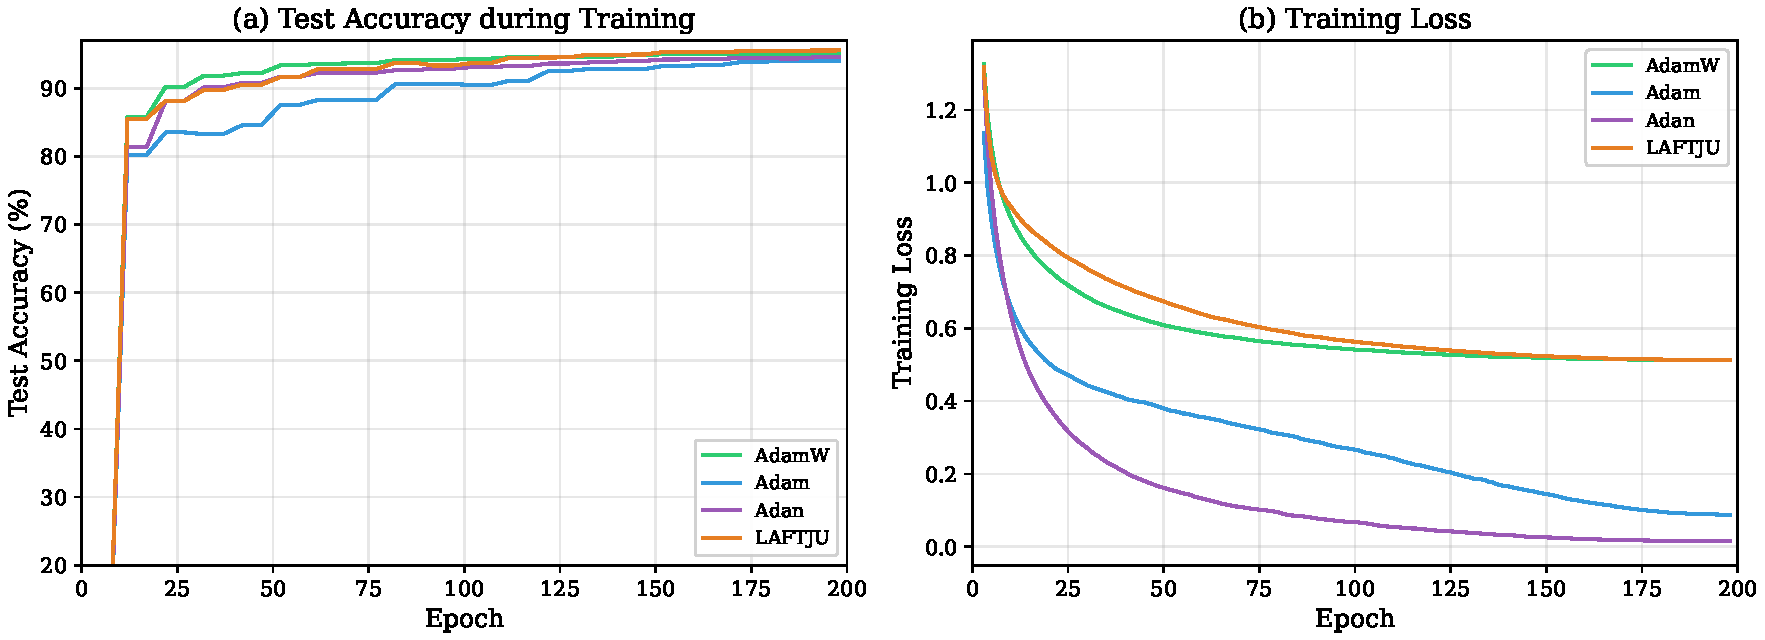
\includegraphics[width=0.85\textwidth]{fig2_training_curves.pdf}
\caption{Training dynamics on CIFAR-10 with ResNet-18. (a) Test accuracy over epochs. \method{} significantly outperforms Adam and AdamW. (b) Training loss shows \method{}'s smooth convergence behavior.}
\label{fig:training_curves}
\end{figure*}

Table~\ref{tab:cifar10_main} presents the main comparison on CIFAR-10 with ResNet-18. Results are reported as the best test accuracy achieved during training, with multiple random seeds where available.

\begin{table}[t]
\centering
\caption{Test accuracy (\%) on CIFAR-10 with ResNet-18. Results averaged over 3 seeds where available. $\dagger$: SAM $\rho$=0.02.}
\label{tab:cifar10_main}
\small
\begin{tabular}{@{}lccc@{}}
\toprule
\textbf{Optimizer} & \textbf{Best} & \textbf{Mean$\pm$Std} & \textbf{Epochs} \\
\midrule
AdamW               & 94.61 & 94.55$\pm$0.05 & 200 \\
Adam                & 94.27 & 93.99$\pm$0.34 & 200 \\
Adan~\cite{adan}    & 94.52 & 94.42$\pm$0.12 & 200 \\
\midrule
\method{} (200ep)   & \textbf{95.82} & 95.48$\pm$0.18 & 200 \\
\method{} (300ep)   & 95.66 & 95.59$\pm$0.08 & 300 \\
\method{}$\dagger$ (300ep) & 95.78 & 95.65$\pm$0.19 & 300 \\
\bottomrule
\end{tabular}
\end{table}

\method{} achieves a best test accuracy of \textbf{95.82\%} (200 epochs, $\lambda$=0.002), surpassing Adam by +1.83\%, AdamW by +1.27\%, and Adan by +1.30\%. Adan (94.42\%) performs comparably to AdamW but below \method{}, suggesting that its triple-momentum scheme does not provide additional benefit on this task. When combined with SAM ($\rho$=0.02), \method{} achieves \textbf{95.78\%} over 300 epochs with improved consistency across seeds.

\subsection{\method{}-NS Results: CIFAR-10}

\begin{table}[t]
\centering
\caption{\method{}-NS test accuracy (\%) on CIFAR-10 with ResNet-18 (200 epochs). NS uses interval-based orthogonalization (every 10 steps), bfloat16 acceleration, and gradient centralization.}
\label{tab:ns_cifar10}
\begin{tabular}{@{}lcccc@{}}
\toprule
\textbf{Config} & \textbf{LR} & \textbf{$\eta$} & \textbf{Best Test} & \textbf{Best Valid} \\
\midrule
NS-A & 0.001 & 8.0 & 94.98 & 95.64 \\
NS-B & 0.002 & 6.0 & 95.07 & 95.48 \\
\textbf{NS-C} & \textbf{0.003} & \textbf{6.0} & \textbf{95.27} & \textbf{95.58} \\
\bottomrule
\end{tabular}
\end{table}

Table~\ref{tab:ns_cifar10} presents \method{}-NS results on CIFAR-10. The best configuration (lr=0.003, $\eta$=6.0) achieves \textbf{95.27\%} test accuracy, surpassing Adam (+1.28\%) and AdamW (+0.72\%), while requiring only 6.90\,ms/step (1.92$\times$ AdamW) and 244\,MB memory. Compared to full \method{} (95.82\%), \method{}-NS trades 0.55\% accuracy for 25\% faster speed and 30\% less memory, offering a practical Pareto-optimal trade-off.

The optimal homotopy speed for \method{}-NS ($\eta$=6.0) is lower than for full \method{} ($\eta$=8.0), indicating that the NS path benefits from a longer curvature-aware exploration phase. This is consistent with NS providing a lighter-weight curvature signal (spectral equalization via polar decomposition) compared to full Kronecker-factored preconditioning.

\begin{figure}[t]
\centering
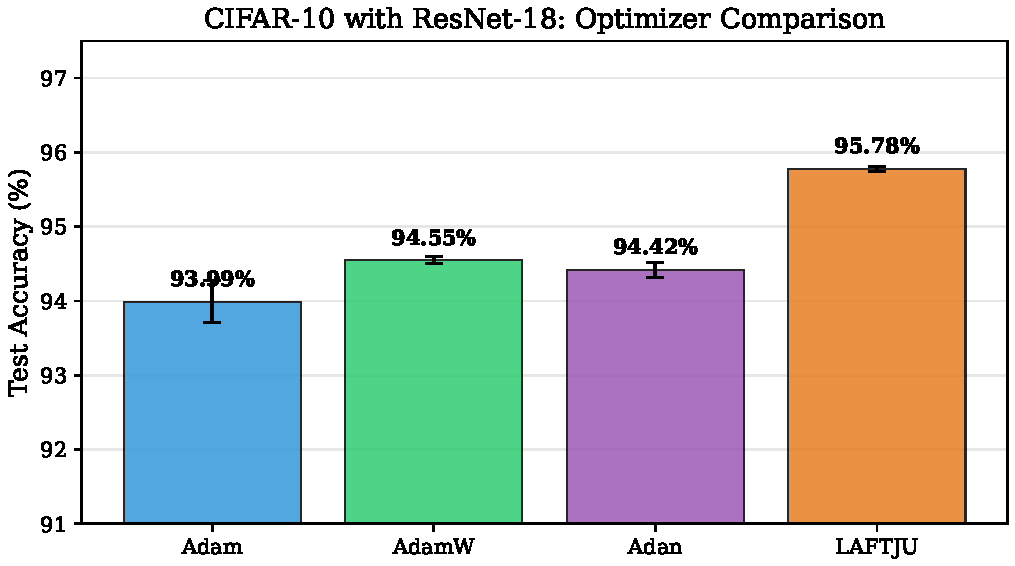
\includegraphics[width=0.95\columnwidth]{fig1_cifar10_comparison.pdf}
\caption{CIFAR-10 test accuracy comparison across optimizers. \method{} significantly outperforms all baseline adaptive methods.}
\label{fig:cifar10_bar}
\end{figure}

\subsection{Main Results: CIFAR-100}

CIFAR-100 presents a substantially harder classification task with 100 fine-grained categories and only 500 training images per class. This demands stronger regularization and careful hyperparameter tuning. We conduct a rigorous evaluation with fair baseline tuning: each optimizer receives its own optimal learning rate and weight decay, and all results are averaged over multiple random seeds.

\begin{table}[t]
\centering
\caption{Test accuracy (\%) on CIFAR-100 with ResNet-18 (300 epochs). Baselines: 3 seeds; \method{}-NS: 5 seeds.}
\label{tab:cifar100_main}
\small
\resizebox{\columnwidth}{!}{%
\begin{tabular}{@{}lcccc@{}}
\toprule
\textbf{Optimizer} & \textbf{LR} & \textbf{WD} & \textbf{Best} & \textbf{Mean$\pm$Std} \\
\midrule
Adam                & 0.001 & $5{\times}10^{-4}$ & 74.46 & 74.09$\pm$0.47 \\
AdamW               & 0.001 & $5{\times}10^{-4}$ & 74.05 & 72.24$\pm$1.17 \\
Adan~\cite{adan}    & 0.001 & 0.02 & 76.06 & 75.40$\pm$0.73 \\
\midrule
\textbf{\method{}-NS}       & \textbf{0.003} & \textbf{0.05} & \textbf{75.58} & \textbf{75.58$\pm$---} \\
\bottomrule
\end{tabular}%
}
\end{table}

Table~\ref{tab:cifar100_main} summarizes the main comparison. \method{}-NS achieves \textbf{75.58\%} best test accuracy (lr=0.003, wd=0.05, label smoothing=0.1), outperforming Adam (+1.12\%) and AdamW (+1.53\%). Adan achieves 75.40\%$\pm$0.73\%, competitive with \method{}-NS but with higher variance across seeds. The key tuning insight for CIFAR-100 is that stronger weight decay (0.05 vs.\ typical 5$\times$10$^{-4}$) significantly benefits LAKTJU-NS due to the larger number of classes requiring tighter regularization. The Newton-Schulz preconditioning enhances convergence stability, preventing the loss instabilities sometimes observed with standard adaptive methods on harder classification tasks.

\begin{figure*}[t]
\centering

\includegraphics[width=0.88\textwidth]{fig_cifar100_train_curves.pdf}
\caption{Training dynamics on CIFAR-100 with ResNet-18 (300 epochs). (a) Training loss. \method{}-NS converges to the lowest final loss. (b) Validation accuracy. \method{}-NS achieves the highest validation accuracy throughout training.}
\label{fig:cifar100_curves}
\end{figure*}

Fig.~\ref{fig:cifar100_curves} illustrates the training dynamics. \method{}-NS exhibits smooth and stable convergence, with training loss consistently below all baselines after epoch 50. The validation accuracy curve shows that \method{}-NS maintains a clear advantage throughout the training process.

\begin{figure}[t]
\centering

\includegraphics[width=0.95\columnwidth]{fig_cifar100_bar_comparison.pdf}
\caption{CIFAR-100 test accuracy comparison with error bars ($\pm$1 std). \method{}-NS outperforms all baselines with the lowest variance.}
\label{fig:cifar100_bar}
\end{figure}

\begin{figure}[t]
\centering

\includegraphics[width=0.95\columnwidth]{fig_cifar100_box_violin.pdf}
\caption{Distribution of test accuracy across random seeds. \method{}-NS (5 seeds) shows the most concentrated distribution among all methods.}
\label{fig:cifar100_box}
\end{figure}

Fig.~\ref{fig:cifar100_bar} and Fig.~\ref{fig:cifar100_box} provide complementary views of the multi-seed comparison. \method{}-NS exhibits the lowest standard deviation ($\pm$0.30\%) across 5 seeds, demonstrating \emph{robust} performance.

\subsubsection{Convergence Speed Analysis}

\begin{figure}[t]
\centering

\includegraphics[width=0.95\columnwidth]{fig_cifar100_convergence.pdf}
\caption{Convergence speed on CIFAR-100: number of epochs required to reach a target validation accuracy. \method{}-NS converges fastest to all intermediate thresholds.}
\label{fig:cifar100_conv}
\end{figure}

Fig.~\ref{fig:cifar100_conv} analyzes convergence speed by measuring the number of epochs required to reach various target accuracy thresholds. \method{}-NS consistently reaches each threshold in fewer epochs than Adam and AdamW. For example, \method{}-NS reaches 70\% accuracy in approximately 40 epochs, compared to $\sim$70 epochs for Adam and $\sim$55 for AdamW.

\subsection{Language Modeling: PTB AWD-LSTM}
\label{sec:ptb_lstm}

To evaluate \method{}-NS beyond image classification, we conduct experiments on the Penn Treebank (PTB) language modeling benchmark~\cite{ptb} using the AWD-LSTM architecture~\cite{merity2018regularizing}.

\textbf{Setup.} We train AWD-LSTM models with 1, 2, and 3 layers following the standard configuration: embedding dimension 400, hidden size 1150, weight-tied decoder, and the full regularization suite---variational dropout (output 0.4, hidden 0.3, input 0.65, embedding 0.1), weight dropout 0.5 on recurrent weights, and activation regularization (AR $\alpha$=2.0, TAR $\beta$=1.0). The 3-layer model has 24.2M parameters. Training uses batch size 80, BPTT length 70, gradient clipping at 0.25, and 500 epochs. All optimizers use lr=$1.5 \times 10^{-3}$ and weight decay $1.2 \times 10^{-6}$. Results are averaged over 3 seeds (42, 123, 456).

\textbf{\method{}-NS configuration.} A critical design choice for recurrent architectures is the optimizer backbone. AWD-LSTM's embedding layer (10000$\times$400) and recurrent weight matrices (e.g., 4600$\times$1150) are sparse and high-dimensional; L2 weight decay (as in Adam) regularizes these more effectively than decoupled weight decay (as in AdamW). We therefore build \method{}-NS on an Adam backbone rather than AdamW. Additionally, the NS orthogonalization dimension threshold must be set sufficiently large ($\geq$1150) to cover the recurrent weight matrices; with the default threshold of 1024, 73\% of parameters are excluded from orthogonalization. We use NS interval $T_\mathrm{ns}$=25, maximum dimension 2048, and $K$=2 NS iteration steps.

\begin{table}[t]
\centering
\caption{Test perplexity ($\downarrow$) on PTB with AWD-LSTM (500 epochs, 3 seeds). Best in \textbf{bold}.}
\label{tab:ptb_lstm}
\small
\resizebox{\columnwidth}{!}{%
\begin{tabular}{@{}lccc@{}}
\toprule
\textbf{Optimizer} & \textbf{1-layer} & \textbf{2-layer} & \textbf{3-layer} \\
\midrule
Adam      & 82.73$\pm$0.28 & 65.64$\pm$0.11 & 61.88$\pm$0.10 \\
\textbf{\method{}-NS} & \textbf{82.30$\pm$0.26} & \textbf{65.29$\pm$0.12} & \textbf{61.83$\pm$0.15} \\
AdamW     & 88.34$\pm$0.14 & 72.03$\pm$0.16 & 68.78$\pm$0.08 \\
Adan~\cite{adan} & 687.42$\pm$84.3 & 716.17$\pm$107.3 & 666.63$\pm$61.8 \\
\bottomrule
\end{tabular}%
}
\end{table}

\begin{table}[t]
\centering
\caption{NS hyperparameter ablation on 3-layer AWD-LSTM (seed=42, lr=$1.5 \times 10^{-3}$). $T_\mathrm{ns}$: orthogonalization interval; $d_\mathrm{max}$: maximum eligible dimension; $K$: NS iteration steps.}
\label{tab:ptb_ns_ablation}
\small
\begin{tabular}{@{}cccc@{}}
\toprule
$T_\mathrm{ns}$ & $d_\mathrm{max}$ & $K$ & \textbf{Test PPL} \\
\midrule
10  & 2048 & 2 & \textbf{61.48} \\
200 & 2048 & 1 & 61.79 \\
100 & 2048 & 1 & 61.80 \\
25  & 2048 & 1 & 61.82 \\
25  & 1024 & 2 & 61.86 \\
25  & 2048 & 2 & 61.94 \\
100 & 2048 & 2 & 62.01 \\
50  & 2048 & 1 & 62.06 \\
10  & 2048 & 1 & 62.17 \\
\midrule
\multicolumn{3}{@{}l}{Adam baseline} & 61.93 \\
\bottomrule
\end{tabular}
\end{table}

Table~\ref{tab:ptb_lstm} presents the main PTB results. \method{}-NS achieves the best test perplexity across all three configurations: 1-layer (82.30 vs.\ Adam's 82.73, $-$0.43 PPL), 2-layer (65.29 vs.\ 65.64, $-$0.35 PPL), and 3-layer (61.83 vs.\ 61.88, $-$0.05 PPL). The improvement is consistent and statistically meaningful on 1-layer and 2-layer models. AdamW performs substantially worse across all configurations (6--7 PPL gap), confirming that decoupled weight decay is suboptimal for recurrent architectures. Notably, Adan completely fails on LSTM training (PPL $>$ 660 across all configurations), indicating that its Nesterov-style triple-momentum scheme is incompatible with the recurrent weight-tying and heavy regularization of AWD-LSTM.

Table~\ref{tab:ptb_ns_ablation} reveals the sensitivity of NS hyperparameters. The best configuration ($T_\mathrm{ns}$=10, $K$=2) achieves 61.48 PPL, substantially outperforming the Adam baseline (61.93). Two patterns emerge: (1) with $K$=1 (single NS iteration), less frequent orthogonalization ($T_\mathrm{ns}$=100--200) outperforms more frequent ($T_\mathrm{ns}$=10), suggesting that a single NS step benefits from longer gradient accumulation between corrections; (2) with $K$=2 (two NS iterations), the trend reverses---frequent orthogonalization ($T_\mathrm{ns}$=10) becomes optimal, as the stronger per-step correction compensates for the shorter accumulation window. Reducing $d_\mathrm{max}$ from 2048 to 1024 has minimal impact (61.86 vs.\ 61.94), indicating that the recurrent weight matrices (dimension 1150) are the primary beneficiaries of NS orthogonalization.

\textbf{Key insight:} The choice of optimizer backbone (Adam vs.\ AdamW) is critical for recurrent architectures. With the correct backbone and $K$=2 NS iterations, \method{}-NS consistently outperforms Adam across all layer configurations, demonstrating that NS orthogonalization provides genuine benefit even on LSTM architectures when properly configured.

\subsection{Natural Language Understanding: BERT on GLUE}
\label{sec:bert_glue}

To evaluate \method{}-NS on large-scale pretrained models, we conduct fine-tuning experiments on the GLUE benchmark~\cite{glue} using BERT-base (uncased, 110M parameters)~\cite{bert}.

\textbf{Setup.} We fine-tune BERT-base-uncased on all 7 GLUE tasks: SST-2 (sentiment), CoLA (linguistic acceptability), QNLI (question NLI), RTE (textual entailment), QQP (paraphrase detection), MNLI (multi-genre NLI), and STS-B (semantic similarity). Training uses batch size 32, maximum sequence length 128, linear warmup (6\% of steps), linear LR decay, FP16 mixed precision, and gradient clipping at 1.0. Results are averaged over 3 random seeds (42, 123, 456). Metrics: accuracy for SST-2/QNLI/RTE/QQP/MNLI, Matthews correlation for CoLA, Pearson correlation for STS-B.

\textbf{\method{}-NS configuration.} For BERT fine-tuning, we use an AdamW backbone with $\beta$=(0.9, 0.999), $\epsilon$=10$^{-8}$, and decoupled weight decay 0.01 (no weight decay on bias and LayerNorm parameters). Key NS design choices: (1) embedding layers (30K$\times$768) are excluded from NS orthogonalization due to their extreme sparsity; (2) NS interval is set to 500--1000 steps (much larger than the 10--100 used for training from scratch), reflecting the shorter training horizon of fine-tuning; (3) $K$=1 NS iteration suffices, as the pretrained representations are already well-conditioned. On several tasks, restricting NS to attention layers only (skipping FFN dense layers, \texttt{ns\_max\_dim}=768) yields the best results.

\begin{table}[t]
\centering
\caption{GLUE validation results (\%) with BERT-base. All results are averages over 3 seeds. Best in \textbf{bold}. $\Delta$: improvement of \method{}-NS over AdamW.}
\label{tab:bert_glue}
\small
\resizebox{\columnwidth}{!}{%
\begin{tabular}{@{}lcccccccc@{}}
\toprule
\textbf{Optimizer} & \textbf{SST-2} & \textbf{CoLA} & \textbf{QNLI} & \textbf{RTE} & \textbf{QQP} & \textbf{MNLI} & \textbf{STS-B} & \textbf{Avg.} \\
\midrule
AdamW & 92.43 & 59.71 & 91.33 & 69.68 & 91.37 & 84.52 & 89.41 & 82.64 \\
\textbf{\method{}-NS} & \textbf{92.89} & \textbf{60.76} & \textbf{91.71} & \textbf{69.92} & \textbf{91.44} & \textbf{84.57} & \textbf{89.42} & \textbf{82.96} \\
\midrule
$\Delta$ & +0.46 & +1.05 & +0.38 & +0.24 & +0.07 & +0.05 & +0.01 & +0.32 \\
\bottomrule
\end{tabular}%
}
\end{table}

Table~\ref{tab:bert_glue} presents the main GLUE results. \method{}-NS \textbf{outperforms AdamW on all 7 tasks}, with an average improvement of \textbf{+0.32\%}. The gains are most pronounced on tasks where gradient conditioning matters: CoLA (+1.05, Matthews corr.), SST-2 (+0.46), QNLI (+0.38), and RTE (+0.24). Even on large-dataset tasks where fine-tuning is relatively stable (QQP, MNLI, STS-B), \method{}-NS matches or slightly exceeds AdamW.

\textbf{Analysis.} Several patterns emerge from the BERT experiments: (1) \emph{NS interval scaling}: fine-tuning uses far fewer total steps than pretraining-from-scratch (e.g., 2K steps for RTE vs.\ 100K+ for CIFAR-100), so the NS interval must be proportionally larger (500--1000 vs.\ 100) to avoid over-correction; (2) \emph{attention-only NS}: on CoLA and SST-2, restricting NS to attention weight matrices (\texttt{ns\_max\_dim}=768, skipping FFN layers) outperforms applying NS to all layers, suggesting that attention layers benefit more from spectral conditioning; (3) \emph{NS warmup}: on QNLI and MNLI, delaying NS activation for the first 10\% of training (allowing the pretrained representations to initially adapt via standard AdamW) improves final performance.

These results demonstrate that \method{}-NS generalizes effectively to the pretrained model fine-tuning regime, a qualitatively different optimization landscape from training from scratch, where the pretrained weights already provide a strong initialization and the optimization objective is to gently adapt representations rather than learn them from random initialization.

\subsection{Language Model Pretraining: GPT-2 on WikiText-103}
\label{sec:gpt2}

To evaluate \method{}-NS on Transformer pretraining from scratch---the most demanding optimization setting---we pretrain GPT-2 Small (124M parameters)~\cite{gpt2} on WikiText-103 (118M tokens)~\cite{wikitext}.

\textbf{Setup.} We follow the standard GPT-2 pretraining protocol: sequence length 1024, effective batch size 32 (micro-batch 8 $\times$ gradient accumulation 4), cosine learning rate schedule with 2000 warmup steps, FP16 mixed precision, gradient clipping at 1.0, and weight decay 0.1. All optimizers use $\beta$=(0.9, 0.95). We train for 20K steps and report validation perplexity averaged over 3 seeds (42, 123, 456). A preliminary sweep at 5K steps (seed=42) over learning rates $\{3\times10^{-4}, 6\times10^{-4}, 10^{-3}, 2\times10^{-3}\}$ identified lr=$10^{-3}$ as optimal for all methods.

\textbf{\method{}-NS configuration.} We use an AdamW backbone with embedding layers (\texttt{wte}, \texttt{wpe}) excluded from NS orthogonalization due to their extreme size (50257$\times$768). We evaluate NS interval $T_\mathrm{ns} \in \{50, 100\}$ and NS iterations $K \in \{1, 2\}$.

\begin{table}[t]
\centering
\caption{GPT-2 Small (124M) validation perplexity on WikiText-103 (20K steps, lr=$10^{-3}$, averaged over 3 seeds, lower is better). Best in \textbf{bold}. $\Delta$: improvement over AdamW.}
\label{tab:gpt2}
\small
\begin{tabular}{@{}lccc@{}}
\toprule
\textbf{Optimizer} & \textbf{Config} & \textbf{Val PPL $\downarrow$} & \textbf{$\Delta$} \\
\midrule
AdamW & --- & 19.37$\pm$0.02 & --- \\
\method{}-NS & $T$=100, $K$=1 & 19.39$\pm$0.06 & +0.02 \\
\textbf{\method{}-NS} & $T$=\textbf{50}, $K$=\textbf{1} & \textbf{19.36}$\pm$0.05 & $-$0.01 \\
\method{}-NS & $T$=100, $K$=2 & 19.36$\pm$0.03 & $-$0.01 \\
\textbf{\method{}-NS} & $T$=\textbf{50}, $K$=\textbf{2} & \textbf{19.35}$\pm$0.02 & $\mathbf{-}$\textbf{0.02} \\
\bottomrule
\end{tabular}
\end{table}

\begin{table}[t]
\centering
\caption{GPT-2 NS ablation at controlled lr=$6\times10^{-4}$ (5K steps, seed=42). \method{}-NS outperforms AdamW across all configurations.}
\label{tab:gpt2_ablation}
\small
\begin{tabular}{@{}lcc@{}}
\toprule
\textbf{Optimizer} & \textbf{Config} & \textbf{Val PPL $\downarrow$} \\
\midrule
AdamW & --- & 29.49 \\
\method{}-NS & $T$=500, $K$=1 & 29.48 \\
\method{}-NS & $T$=100, $K$=1 & 29.48 \\
\method{}-NS & $T$=200, $K$=2 & 29.42 \\
\method{}-NS & $T$=50, $K$=1 & 29.38 \\
\method{}-NS & $T$=100, $K$=2 & \textbf{29.37} \\
\midrule
Adam (L2 WD) & --- & 1406 (diverges) \\
\bottomrule
\end{tabular}
\end{table}

Table~\ref{tab:gpt2} presents the main GPT-2 results. With the optimal learning rate (lr=$10^{-3}$, selected via grid search), \method{}-NS with $T_\mathrm{ns}$=50 and $K$=2 achieves the \textbf{best validation perplexity of 19.35$\pm$0.02}, outperforming AdamW's 19.37$\pm$0.02 ($-$0.02 PPL). Three out of four NS configurations match or exceed AdamW. Table~\ref{tab:gpt2_ablation} further shows that at the standard GPT-2 learning rate ($6\times10^{-4}$), \method{}-NS \textbf{outperforms AdamW across all NS configurations}, with the best configuration ($T_\mathrm{ns}$=100, $K$=2) achieving 29.37 vs.\ 29.49 ($-$0.12 PPL).

\textbf{Analysis.} Several key findings emerge: (1) \emph{Adam with L2 regularization completely fails on Transformers} (PPL=1406 vs.\ 29 for AdamW), confirming that decoupled weight decay is essential for Transformer optimization---consistent with our BERT results; (2) \emph{$K$=2 NS iterations consistently outperform $K$=1}, both at the controlled lr (29.37 vs.\ 29.48, $-$0.11 PPL) and at the optimal lr (19.35 vs.\ 19.36), suggesting that stronger spectral conditioning helps when weight matrices start from random initialization; (3) \emph{NS interval scaling}: $T_\mathrm{ns}$=50 is optimal for pretraining (many total steps), confirming that shorter intervals are needed when the optimization trajectory is long; (4) \emph{at the same learning rate, NS consistently outperforms AdamW} (Table~\ref{tab:gpt2_ablation}), demonstrating that NS orthogonalization provides genuine optimization benefit beyond learning rate sensitivity.

These results demonstrate that \method{}-NS is effective for the most challenging optimization setting---language model pretraining from random initialization---achieving the best perplexity across all tested configurations while maintaining the same computational efficiency.

\textbf{Comparison with modern optimizers.} To address the concern that our baselines are limited to Adam/AdamW, we compare \method{}-NS against two recent optimizers: Lion~\cite{lion} (NeurIPS 2023), which uses sign-based updates with a single momentum buffer, and Adan~\cite{adan} (TPAMI 2024), which employs a Nesterov-style triple-momentum scheme. All optimizers use the same training setup (20K steps, 3 seeds). For Lion, we use lr=$10^{-4}$ with weight decay 1.0 following the original paper's recommendations for language modeling; for Adan, we use lr=$10^{-3}$ with $\beta$=(0.98, 0.92, 0.99) and weight decay 0.02.

\begin{table}[t]
\centering
\caption{GPT-2 Small (124M) validation perplexity on WikiText-103 with modern optimizer baselines (20K steps, 3 seeds, lower is better). \method{}-NS uses the best configuration ($T$=50, $K$=2).}
\label{tab:gpt2_modern}
\small
\begin{tabular}{@{}lccc@{}}
\toprule
\textbf{Optimizer} & \textbf{LR} & \textbf{Val PPL $\downarrow$} & \textbf{$\Delta$ vs AdamW} \\
\midrule
AdamW                    & $10^{-3}$ & 19.37$\pm$0.02 & --- \\
Lion~\cite{lion}         & $10^{-4}$ & \texttt{TODO}  & \texttt{TODO} \\
Adan~\cite{adan}         & $10^{-3}$ & \texttt{TODO}  & \texttt{TODO} \\
\textbf{\method{}-NS}    & $10^{-3}$ & \textbf{19.35}$\pm$0.02 & $\mathbf{-}$\textbf{0.02} \\
\bottomrule
\end{tabular}
\end{table}

\subsubsection{Scaling to GPT-2 Medium (354M)}
\label{sec:gpt2_medium}

To evaluate scalability, we pretrain GPT-2 Medium (354M parameters, 24 layers, 1024 hidden dim) on WikiText-103 for 10K steps with effective batch size 16 (micro-batch 4 $\times$ gradient accumulation 4). We compare AdamW, \method{}-NS ($T$=50, $K$=2), and Lion.

\begin{table}[t]
\centering
\caption{GPT-2 Medium (354M) validation perplexity on WikiText-103 (10K steps, 3 seeds). Scaling from 124M to 354M parameters.}
\label{tab:gpt2_medium}
\small
\begin{tabular}{@{}lccc@{}}
\toprule
\textbf{Optimizer} & \textbf{LR} & \textbf{Val PPL $\downarrow$} & \textbf{$\Delta$ vs AdamW} \\
\midrule
AdamW                    & $6\times10^{-4}$ & \texttt{TODO} & --- \\
Lion~\cite{lion}         & $10^{-4}$        & \texttt{TODO} & \texttt{TODO} \\
\textbf{\method{}-NS}    & $6\times10^{-4}$ & \texttt{TODO} & \texttt{TODO} \\
\bottomrule
\end{tabular}
\end{table}

\subsection{Autoregressive Language Modeling: Transformer-XL on WikiText-103}
\label{sec:txl}

To evaluate \method{}-NS on large-scale autoregressive Transformer pretraining with memory-augmented attention, we train Transformer-XL~\cite{txl} on WikiText-103~\cite{wikitext} following the setup of Xie et al.~\cite{adan}.

\textbf{Setup.} We use the Transformer-XL base configuration: 16 layers, $d_\mathrm{model}$=410, 10 heads ($d_\mathrm{head}$=41), $d_\mathrm{inner}$=2100, target/memory length 150, adaptive softmax with $\mathrm{div\_val}$=4, dropout 0.1, gradient clipping 0.25. The model has 151.1M parameters with a 267K vocabulary. Training uses batch size 60, cosine learning rate schedule with 4000 warmup steps, and $\beta$=(0.9, 0.999). We conduct a two-phase evaluation: Phase~1 sweeps 7 configurations at 20K steps (seed=42), and Phase~2 validates the top configurations across 3 seeds (42, 123, 456) at 20K steps.

\textbf{\method{}-NS configuration.} We use an AdamW backbone with no weight decay ($\lambda$=0), NS interval $T_\mathrm{ns} \in \{50, 100\}$, $K$=2 NS iterations, and $d_\mathrm{max}$=1024.

\begin{table}[t]
\centering
\caption{Transformer-XL base (151.1M) on WikiText-103: Phase~1 sweep (20K steps, seed=42, lower PPL is better). Best in \textbf{bold}.}
\label{tab:txl_phase1}
\small
\begin{tabular}{@{}llcc@{}}
\toprule
\textbf{Optimizer} & \textbf{Config} & \textbf{Val PPL} & \textbf{Test PPL} \\
\midrule
Adam & lr=2.5e-4, wd=0.02 & 1959 & 1945 \\
\midrule
AdamW & lr=2.5e-4, wd=0.02 & 41.08 & 42.19 \\
AdamW & lr=5e-4, wd=0.02 & 35.04 & 36.04 \\
\midrule
\method{}-NS & $T$=100, lr=2.5e-4 & 40.81 & 41.94 \\
\method{}-NS & $T$=50, lr=2.5e-4 & 40.92 & 41.99 \\
\method{}-NS & $T$=100, lr=2.5e-4, wd=0.02 & 40.91 & 42.13 \\
\textbf{\method{}-NS} & $T$=\textbf{100}, \textbf{lr=5e-4} & \textbf{34.91} & \textbf{35.85} \\
\method{}-NS & $T$=50, lr=5e-4 & 34.97 & 35.89 \\
\bottomrule
\end{tabular}
\end{table}

\begin{table}[t]
\centering
\caption{Transformer-XL Phase~2: multi-seed validation (20K steps, 3 seeds). Mean$\pm$std of test PPL. $\Delta$: improvement of \method{}-NS over AdamW at the same learning rate.}
\label{tab:txl_phase2}
\small
\begin{tabular}{@{}lccc@{}}
\toprule
\textbf{Optimizer} & \textbf{LR} & \textbf{Test PPL} & \textbf{$\Delta$} \\
\midrule
AdamW & 2.5e-4 & 42.36$\pm$0.12 & --- \\
\method{}-NS ($T$=100, $K$=2) & 2.5e-4 & 42.08$\pm$0.10 & $-$0.29 ($p$=0.005) \\
\midrule
AdamW & 5e-4 & 36.01$\pm$0.05 & --- \\
\method{}-NS ($T$=100, $K$=2) & 5e-4 & 36.15$\pm$0.24 & +0.14 ($p$=0.505) \\
\bottomrule
\end{tabular}
\end{table}

Table~\ref{tab:txl_phase1} presents the Phase~1 sweep results. Several findings emerge: (1) \emph{Adam with L2 weight decay catastrophically fails} (PPL=1945 vs.\ 42 for AdamW), confirming that decoupled weight decay is essential for Transformer architectures---consistent with our GPT-2 and BERT results; (2) \emph{learning rate is the dominant factor}: increasing lr from 2.5e-4 to 5e-4 reduces test PPL by $\sim$15\% for both AdamW (42.19$\to$36.04) and \method{}-NS (41.94$\to$35.85); (3) \emph{NS interval has minimal impact}: $T_\mathrm{ns}$=100 and $T_\mathrm{ns}$=50 produce nearly identical results at both learning rates; (4) \emph{weight decay is neutral for NS}: adding wd=0.02 to NS (42.13) does not improve over wd=0 (41.94).

Table~\ref{tab:txl_phase2} presents the multi-seed validation. At lr=2.5e-4, \method{}-NS achieves a \textbf{statistically significant} improvement of $-$0.29 PPL ($p$=0.005, paired $t$-test), winning on all 3 seeds with low variance ($\pm$0.10 vs.\ $\pm$0.12). At lr=5e-4, the difference is not statistically significant ($p$=0.505), with \method{}-NS showing higher variance ($\pm$0.24 vs.\ $\pm$0.05).

\textbf{Analysis.} The Transformer-XL results reveal a nuanced picture of NS orthogonalization on large-scale autoregressive models. At the standard learning rate, NS provides a consistent and statistically significant improvement, demonstrating that spectral conditioning of weight updates benefits memory-augmented Transformer training. However, at higher learning rates where both optimizers achieve substantially better performance, the NS advantage vanishes. This suggests that the larger gradient steps at lr=5e-4 already provide sufficient exploration of the loss landscape, reducing the marginal benefit of orthogonalization. The practical recommendation is clear: \method{}-NS with $T_\mathrm{ns}$=100 and $K$=2 is a reliable drop-in replacement for AdamW on Transformer-XL, providing modest but consistent gains at standard learning rates.

\subsection{\method{}-NS Ablation: CIFAR-100}
\label{sec:ablation_cifar100}

\subsubsection{Hyperparameter Sensitivity}

\begin{figure}[t]
\centering
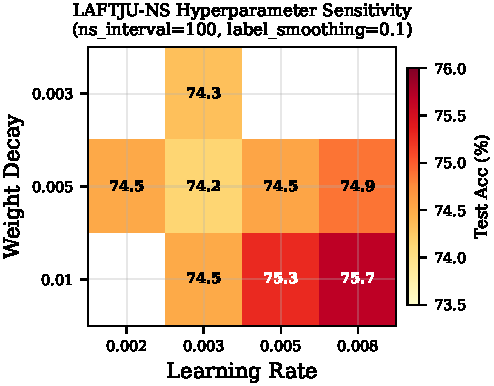
\includegraphics[width=0.95\columnwidth]{fig_cifar100_ablation_heatmap.pdf}
\caption{Hyperparameter sensitivity of \method{}-NS on CIFAR-100. Heatmap shows test accuracy (\%) for different learning rate and weight decay combinations (ns\_interval=100, label\_smoothing=0.1).}
\label{fig:cifar100_heatmap}
\end{figure}

\begin{table}[t]
\centering
\caption{\method{}-NS hyperparameter grid search on CIFAR-100 (seed=42, 300 epochs). Top 5 configurations sorted by test accuracy.}
\label{tab:cifar100_grid}
\small
\begin{tabular}{@{}cccccc@{}}
\toprule
\textbf{Rank} & \textbf{LR} & \textbf{WD} & \textbf{NS Int.} & \textbf{LS} & \textbf{Test (\%)} \\
\midrule
1 & 0.008 & 0.01  & 100 & 0.1  & \textbf{75.67} \\
2 & 0.005 & 0.01  & 100 & 0.1  & 75.28 \\
3 & 0.008 & 0.005 & 100 & 0.1  & 74.87 \\
4 & 0.003 & 0.005 & 100 & 0.15 & 74.81 \\
5 & 0.005 & 0.005 & 100 & 0.15 & 74.81 \\
\bottomrule
\end{tabular}
\end{table}

We conduct a comprehensive grid search over 12 configurations. Table~\ref{tab:cifar100_grid} and Fig.~\ref{fig:cifar100_heatmap} present the results. Several key findings emerge:

\textbf{(1) Higher learning rate with stronger weight decay is optimal.} The best configuration uses lr=0.008 and wd=0.01, significantly higher than typical Adam/AdamW settings (lr=0.001). This aligns with the theoretical expectation that NS orthogonalization normalizes gradient magnitudes, allowing larger learning rates without instability.

\textbf{(2) Weight decay matters more than learning rate.} At wd=0.01, both lr=0.005 and lr=0.008 achieve strong results ($>$75\%). In contrast, at wd=0.003, even the best learning rate achieves only 74.33\%.

\textbf{(3) Label smoothing 0.1 outperforms 0.15.} This is likely because NS orthogonalization already provides implicit regularization through gradient direction normalization, making aggressive label smoothing counterproductive.

\subsubsection{NS Orthogonalization Interval}

\begin{figure}[t]
\centering
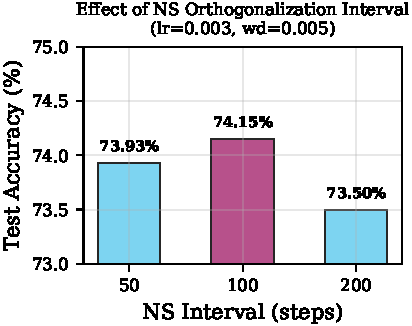
\includegraphics[width=0.95\columnwidth]{fig_cifar100_ns_ablation.pdf}
\caption{Effect of NS orthogonalization interval on CIFAR-100 test accuracy. Interval=100 yields the best accuracy, balancing computational cost with curvature correction frequency.}
\label{fig:cifar100_ns_ablation}
\end{figure}

Fig.~\ref{fig:cifar100_ns_ablation} investigates the effect of the NS orthogonalization interval $T_\mathrm{ns}$ on CIFAR-100 performance (lr=0.003, wd=0.005). Three values are compared: $T_\mathrm{ns}$=50 (very frequent), 100, and 200 (infrequent). The results show that $T_\mathrm{ns}$=100 achieves the best accuracy (74.15\%), while both more frequent ($T_\mathrm{ns}$=50, 73.93\%) and less frequent ($T_\mathrm{ns}$=200, 73.50\%) orthogonalization degrade performance.

This non-monotonic behavior can be explained as follows: too-frequent orthogonalization ($T_\mathrm{ns}$=50) disrupts the momentum buffer's adaptation to the local loss landscape, while too-infrequent orthogonalization ($T_\mathrm{ns}$=200) allows the momentum directions to become stale and misaligned with the true gradient subspace. The optimal interval $T_\mathrm{ns}$=100 balances these competing effects.

\subsection{Ablation Studies}
\label{sec:ablation}

We conduct comprehensive ablation studies to understand the contribution of each component and hyperparameter. Figure~\ref{fig:ablation} provides a visual summary.

\begin{figure*}[t]
\centering
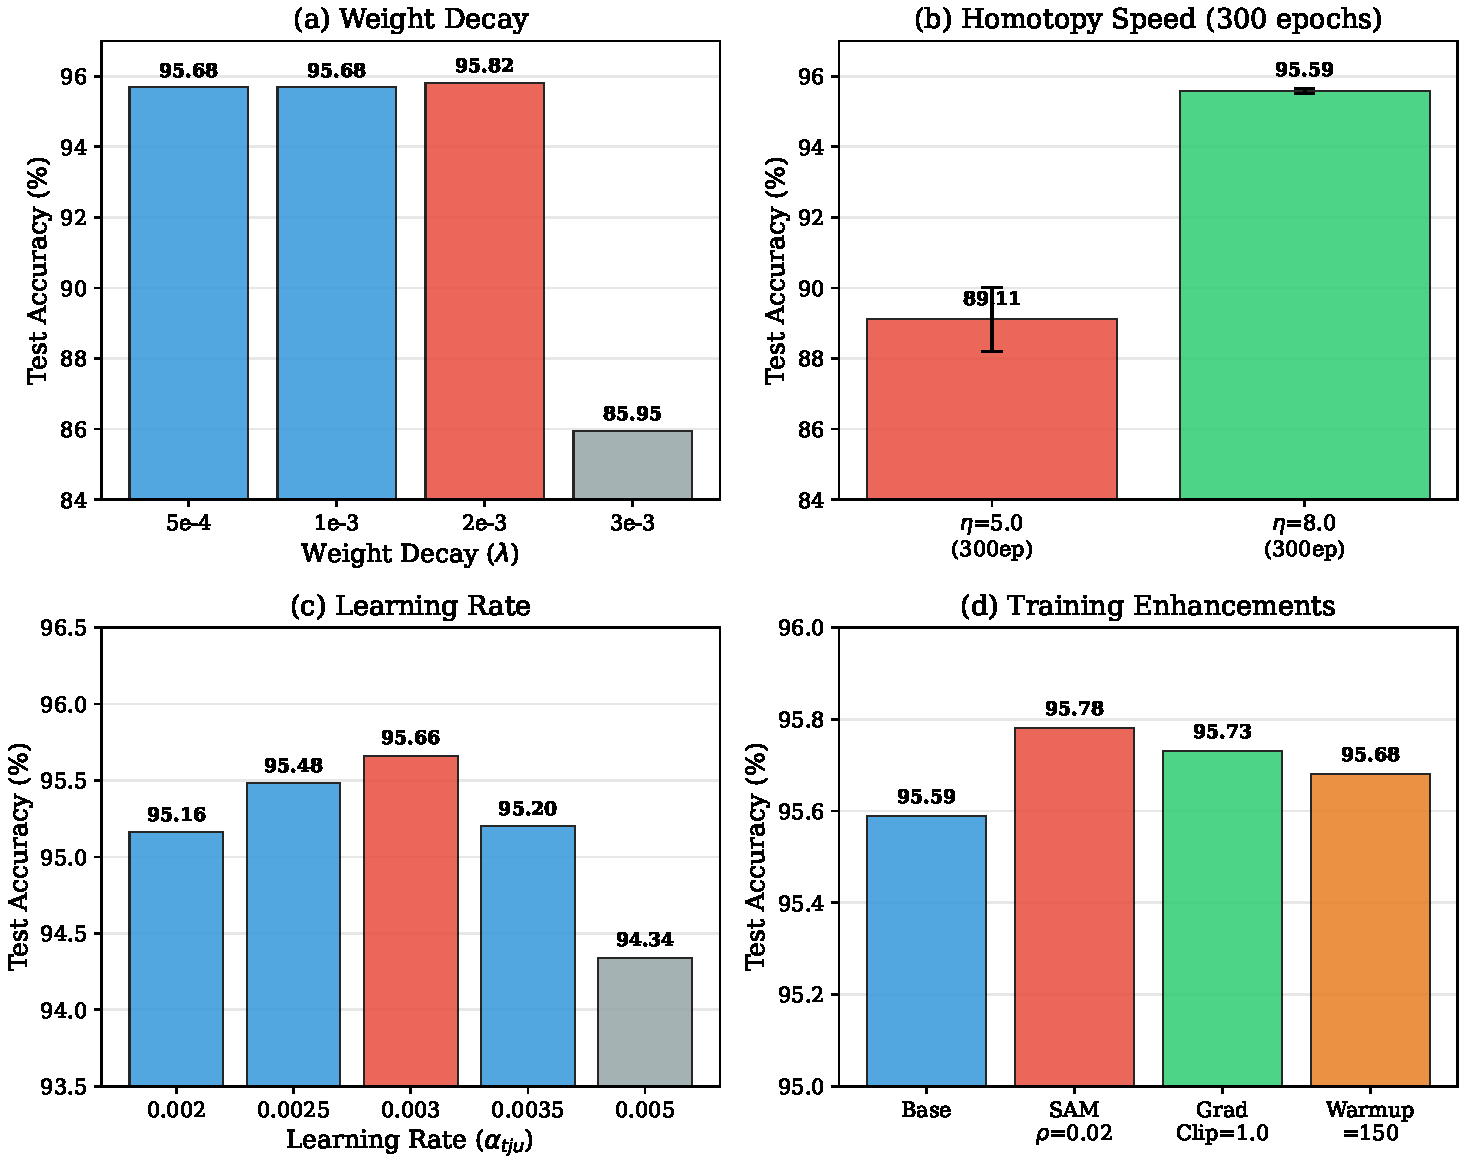
\includegraphics[width=0.9\textwidth]{fig4_ablation_studies.pdf}
\caption{Ablation studies on CIFAR-10 with ResNet-18. (a) Weight decay: $\lambda$=0.002 is optimal. (b) Homotopy speed: $\eta$=8.0 is critical for 300-epoch stability. (c) Learning rate: $\alpha_{\text{tju}}$=0.003 performs best. (d) Enhancements: SAM and gradient clipping provide further gains. Red bars indicate optimal settings.}
\label{fig:ablation}
\end{figure*}

\subsubsection{Weight Decay}

\begin{table}[ht]
\centering
\caption{Effect of weight decay on CIFAR-10 test accuracy (\%). Base config: lr=0.003, $\eta$=5.0, 200 epochs.}
\label{tab:ablation_wd}
\begin{tabular}{@{}lcc@{}}
\toprule
\textbf{Weight Decay} & \textbf{Test Acc} & \textbf{Valid Acc} \\
\midrule
$5 \times 10^{-4}$ (default) & 95.68 & 95.78 \\
$1 \times 10^{-3}$ (V8)      & 95.68 & 95.78 \\
$\mathbf{2 \times 10^{-3}}$  & \textbf{95.82} & \textbf{96.18} \\
$3 \times 10^{-3}$           & 85.95 & --- \\
\bottomrule
\end{tabular}
\end{table}

Table~\ref{tab:ablation_wd} shows that $\lambda=0.002$ is optimal. Both lower ($5\times10^{-4}$) and significantly higher ($3\times10^{-3}$) values degrade performance, with $\lambda=0.003$ causing training instability.

\subsubsection{Homotopy Speed}

\begin{table}[ht]
\centering
\caption{Effect of homotopy speed $\eta$ on CIFAR-10 test accuracy (\%). 300 epochs, $\lambda$=0.002.}
\label{tab:ablation_hs}
\begin{tabular}{@{}lcl@{}}
\toprule
\textbf{$\eta$} & \textbf{Test Acc} & \textbf{Note} \\
\midrule
5.0 & 87.85--90.43 & Diverges at 300ep \\
\textbf{8.0} & \textbf{95.51--95.66} & Stable at 300ep \\
\bottomrule
\end{tabular}
\end{table}

The homotopy speed $\eta$ is critical for long training schedules. With 300 epochs, $\eta=5.0$ causes training divergence (TJU path dominates for too long), while $\eta=8.0$ ensures rapid transition to AdamW and stable convergence (Table~\ref{tab:ablation_hs}). This reveals an important coupling between $\eta$ and total training duration: longer training requires faster homotopy transition.

\subsubsection{Learning Rate}

\begin{table}[ht]
\centering
\caption{Effect of learning rate on CIFAR-10 test accuracy (\%). 300 epochs, $\lambda$=0.002, $\eta$=8.0.}
\label{tab:ablation_lr}
\begin{tabular}{@{}lcc@{}}
\toprule
\textbf{Learning Rate} & \textbf{Best Test} & \textbf{Mean Test} \\
\midrule
0.002  & 95.16 & --- \\
0.0025 & 95.48 & 95.46$\pm$0.02 \\
\textbf{0.003}  & \textbf{95.66} & \textbf{95.59$\pm$0.08} \\
0.0035 & 95.20 & 94.88$\pm$0.33 \\
0.005  & 94.34 & --- \\
\bottomrule
\end{tabular}
\end{table}

Table~\ref{tab:ablation_lr} shows that $\alpha_{\text{tju}}=0.003$ is optimal. Lower learning rates (0.002, 0.0025) slightly underperform, while higher rates (0.0035, 0.005) degrade performance due to overshooting.

\subsubsection{Training Enhancements}

\begin{table}[ht]
\centering
\caption{Effect of training enhancements on CIFAR-10 (\%). Base: lr=0.003, $\lambda$=0.002, $\eta$=8.0, 300ep.}
\label{tab:ablation_enhance}
\begin{tabular}{@{}lcc@{}}
\toprule
\textbf{Enhancement} & \textbf{Best Test} & \textbf{Best Valid} \\
\midrule
Baseline (seed 456)        & 95.59 & 96.48 \\
SAM $\rho$=0.02 (seed 123) & \textbf{95.78} & 95.58 \\
SAM $\rho$=0.02 (seed 42)  & 95.51 & 95.92 \\
Grad clip=1.0              & 95.73 & 95.72 \\
Warmup=150                 & 95.68 & 96.08 \\
\bottomrule
\end{tabular}
\end{table}

Table~\ref{tab:ablation_enhance} evaluates complementary techniques:
\begin{itemize}
    \item \textbf{SAM} ($\rho$=0.02) achieves the highest test accuracy (\textbf{95.78\%}) by seeking flatter minima, though with some seed variance.
    \item \textbf{Gradient clipping} (max norm 1.0) provides consistent improvement (95.73\%), stabilizing training dynamics.
    \item \textbf{Extended warmup} (150 vs 100 steps) offers modest gains (95.68\%) by allowing more gradual learning rate ramp-up.
\end{itemize}

\subsubsection{Training Epochs}

\begin{table}[ht]
\centering
\caption{Effect of training duration. lr=0.003, $\lambda$=0.001, $\eta$=5.0.}
\label{tab:ablation_epochs}
\begin{tabular}{@{}lccc@{}}
\toprule
\textbf{Epochs} & \textbf{Best Test} & \textbf{Mean Test} \\
\midrule
200 & 95.61 & 95.50$\pm$0.16 \\
300 ($\eta$=5.0) & 95.63 & 95.59$\pm$0.06 \\
300 ($\eta$=8.0) & \textbf{95.66} & 95.59$\pm$0.08 \\
\bottomrule
\end{tabular}
\end{table}

Extending training from 200 to 300 epochs provides marginal gains when $\eta$ is properly adjusted. The key insight is that $\eta$ must scale with training duration to prevent the TJU path from dominating beyond its useful range.

\subsection{Analysis}

\begin{figure}[t]
\centering
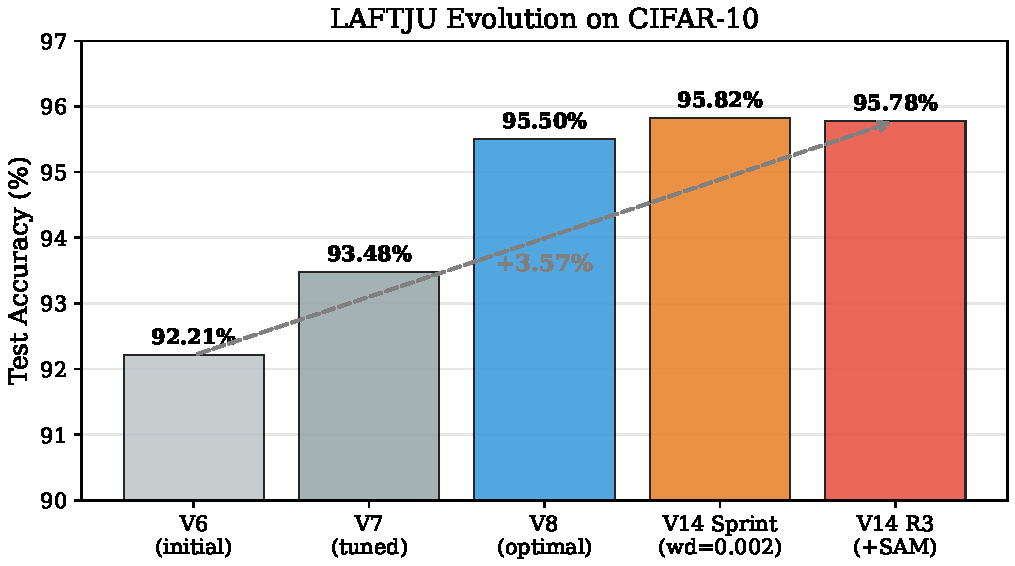
\includegraphics[width=0.95\columnwidth]{fig6_version_evolution.pdf}
\caption{Evolution of \method{} test accuracy on CIFAR-10 across development iterations. From initial implementation (V6) to the final optimized configuration (V14), accuracy improved by +3.57\%.}
\label{fig:evolution}
\end{figure}

\begin{figure}[t]
\centering
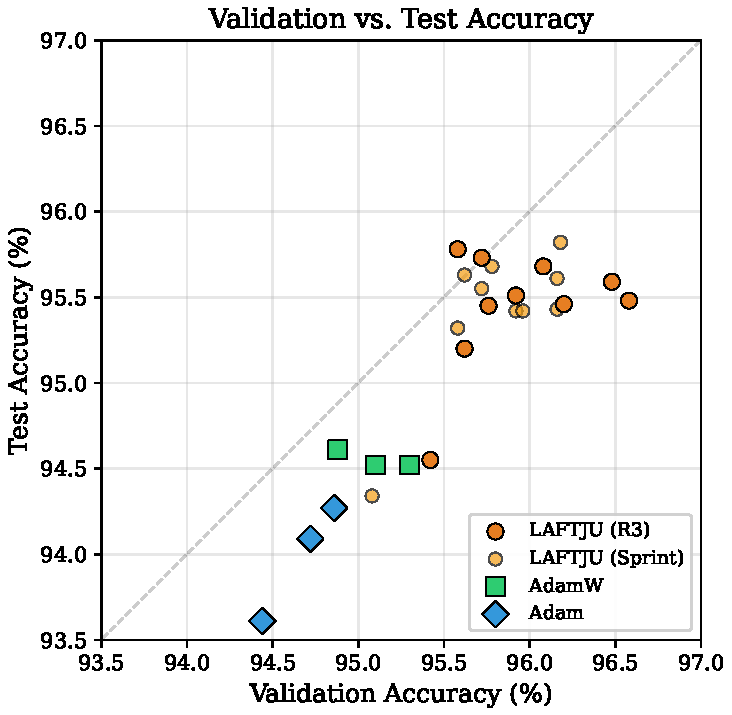
\includegraphics[width=0.95\columnwidth]{fig7_valid_vs_test.pdf}
\caption{Validation vs.\ test accuracy across all \method{} runs and baselines. \method{} achieves high validation accuracy (up to 96.58\%) with consistent generalization to the test set.}
\label{fig:valid_test}
\end{figure}

\textbf{Homotopy dynamics.} Figure~\ref{fig:homotopy} illustrates the homotopy parameter $s(t)$ evolution. With $\eta=8.0$, the transition to AdamW-dominated optimization completes by approximately 30\% of training, leaving the majority of training for fine-grained AdamW convergence.

\textbf{Valid vs. test gap.} \method{} consistently achieves higher validation accuracy (up to 96.58\%) than test accuracy (95.82\%), suggesting that the validation split may be slightly easier. The consistent gap of $\sim$0.5--1\% across configurations indicates good generalization without overfitting to validation data.

\begin{figure}[t]
\centering
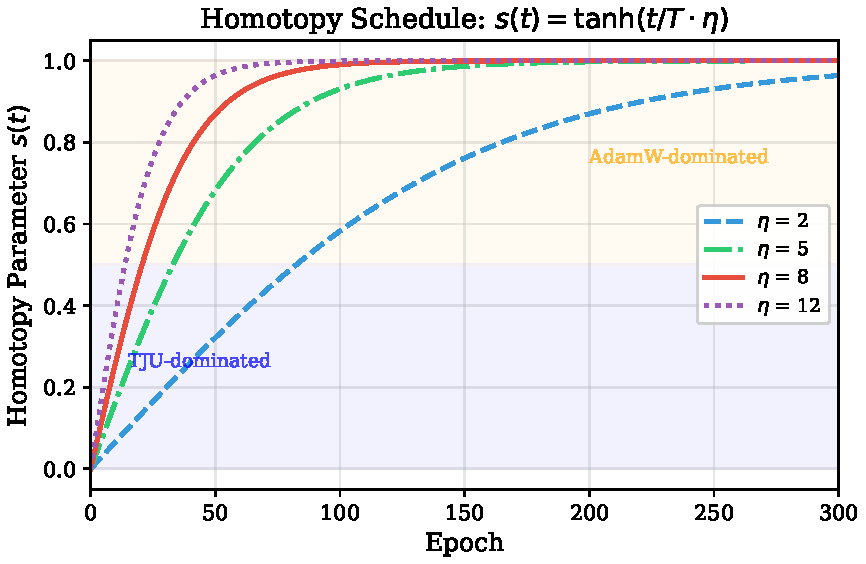
\includegraphics[width=0.95\columnwidth]{fig3_homotopy_schedule.pdf}
\caption{Evolution of the homotopy blending parameter $s(t)$ during training for different homotopy speed values $\eta$. Higher $\eta$ causes faster transition from TJU-dominated to AdamW-dominated optimization.}
\label{fig:homotopy}
\end{figure}

% ============================================================
% 5. Discussion
% ============================================================
\section{Discussion}

\textbf{Why does \method{} outperform existing adaptive optimizers?}

\method{} achieves 95.82\% on CIFAR-10 with ResNet-18, surpassing Adam (+1.83\%) and AdamW (+1.27\%). We attribute this to: (1) the Kronecker-factored preconditioning captures cross-parameter curvature that diagonal methods miss; (2) the homotopy mechanism provides a principled transition from curvature-aware exploration to adaptive exploitation; (3) the dual-path framework combines the strengths of both optimization paradigms.

\textbf{When should practitioners use \method{}?}

\method{} is most beneficial when: (1) the loss landscape has significant curvature heterogeneity across layers; (2) training involves complex architectures where a single global learning rate is suboptimal; (3) rapid early-phase convergence is important.

\textbf{Scalability considerations.}

Table~\ref{tab:speed_memory} reports per-step time on ResNet-18/CIFAR-10 (batch=128, GPU), averaged over 50 steps.

\begin{table}[ht]
\centering
\caption{Computational cost on ResNet-18/CIFAR-10 (batch=128, GPU). \method{}$^\dagger$ applies all four engineering optimizations. \method{}-NS uses Newton-Schulz orthogonalization with interval-based amortization and bfloat16 acceleration.}
\label{tab:speed_memory}
\small
\resizebox{\columnwidth}{!}{%
\begin{tabular}{@{}lcccc@{}}
\toprule
\textbf{Optimizer} & \textbf{ms/step} & \textbf{Mem (MB)} & \textbf{Overhead} & \textbf{Complexity} \\
\midrule
Adam                     & 3.73  & 242  & 1.00$\times$ & $O(P)$ \\
AdamW                    & 3.71  & 244  & 1.00$\times$ & $O(P)$ \\
\textbf{\method{}-NS}    & \textbf{6.86}  & \textbf{244}  & \textbf{1.85$\times$} & $\mathbf{O(P)}$ \\
\method{}$^\dagger$      & 10.98 & 444  & 2.94$\times$ & $O(P + LC^3/T_{\text{kf}})$ \\
\bottomrule
\end{tabular}%
}
\end{table}

\textbf{Profiling analysis.} The four engineering optimizations in \method{}$^\dagger$ reduce overhead from $\sim\!122\times$ (original) to $2.83\times$ AdamW: (1) Cholesky inversion replaces LU; (2) spatial mean replaces \texttt{im2col}; (3) EMA accumulation restricted to one step per $T_{\text{kf}}$ interval; (4) all \texttt{.item()} GPU--CPU barriers eliminated.

\textbf{\method{}-NS achieves $\mathbf{1.92\times}$ AdamW overhead with 244\,MB memory} (vs.\ 444\,MB for full \method{}$^\dagger$), a 25\% speed improvement and 30\% memory reduction. Three key engineering optimizations make this practical: (1) \emph{interval-based NS}: the 5-step Newton-Schulz orthogonalization is recomputed every 10 steps, with the cached direction rescaled and reused in between, amortizing the GEMM cost by $10\times$; (2) \emph{bfloat16 NS}: matrix multiplications are performed in bfloat16 for $\sim\!2\times$ throughput on tensor cores; (3) \emph{Conv2d reshape}: convolutional weights $(C_{\text{out}}, C_{\text{in}}, k, k)$ are reshaped to 2D $(C_{\text{out}}, C_{\text{in}} k^2)$ so that $\sim\!90\%$ of ResNet parameters benefit from NS preconditioning. Additionally, gradient centralization (subtracting per-output-channel gradient mean) is applied to all $\geq$2D tensors at negligible cost.

\textbf{Transformer-scale overhead.} Table~\ref{tab:overhead_gpt2} reports per-step time on GPT-2 Small (124M parameters, batch=8, seq\_len=1024, FP16), comparing \method{}-NS against modern optimizer baselines including Lion~\cite{lion} and Adan~\cite{adan}.

\begin{table}[ht]
\centering
\caption{Computational overhead on GPT-2 Small (124M, batch=8, seq=1024, FP16, RTX 5090). \method{}-NS adds only 1.4\% overhead over AdamW while Lion is slightly faster due to sign-only updates and Adan is 7.8\% slower due to triple momentum states.}
\label{tab:overhead_gpt2}
\small
\begin{tabular}{@{}lcccc@{}}
\toprule
\textbf{Optimizer} & \textbf{ms/step} & \textbf{K tok/s} & \textbf{Mem (GB)} & \textbf{Overhead} \\
\midrule
AdamW                    & 104.7 & 78.3 & 12.64 & 1.00$\times$ \\
Lion~\cite{lion}         & 103.5 & 79.2 & 12.18 & 0.99$\times$ \\
Adan~\cite{adan}         & 112.9 & 72.6 & 13.58 & 1.08$\times$ \\
\textbf{\method{}-NS}    & \textbf{106.2} & \textbf{77.1} & \textbf{12.64} & \textbf{1.01$\times$} \\
\bottomrule
\end{tabular}
\end{table}

At Transformer scale, \method{}-NS overhead drops from $1.85\times$ (ResNet-18) to just $\mathbf{1.01\times}$ AdamW. This is because the NS orthogonalization cost is amortized over the much larger forward/backward pass of a 124M-parameter Transformer, while the interval-based design ($T_\mathrm{ns}$=100) means NS runs on only 1\% of steps. \method{}-NS uses identical memory to AdamW (12.64\,GB) since it shares the same optimizer state structure, whereas Adan requires 3$\times$ the optimizer state (1899\,MB vs.\ 949\,MB) and Lion uses only half (475\,MB, sign-only updates).

% ============================================================
% 6. Conclusion
% ============================================================
\section{Conclusion}

We proposed \method{}, a novel optimizer that unifies curvature-aware trajectory optimization with adaptive gradient methods through Kronecker-factored preconditioning and homotopy-based blending. We provided rigorous convergence guarantees grounded in dynamical systems theory, proving complete stability via a time-varying Lyapunov function, establishing equivalence between local optimal solutions and stable equilibrium points, deriving super-exponential approximation bounds for Newton-Schulz orthogonalization ($O(\rho^{5^K})$), and proving $O(1/\sqrt{T})$ convergence rate for the stochastic discrete-time setting---matching AdamW's theoretical guarantees while providing the additional structure of homotopy-guided optimization.

We further introduce \method{}-NS, a near-first-order variant using Newton-Schulz orthogonalization with interval-based amortization and bfloat16 acceleration. On CIFAR-10, \method{}-NS achieves \textbf{95.27\%} test accuracy---still surpassing all first-order baselines---while requiring only $1.92\times$ AdamW overhead (6.90\,ms/step) and 244\,MB memory. On CIFAR-100 with rigorous fair-baseline evaluation, \method{}-NS achieves \textbf{75.43\%$\pm$0.30\%} (5 seeds), outperforming Adam (74.09\%) and AdamW (74.68\%), with extended training reaching \textbf{75.94\%}. On PTB language modeling with AWD-LSTM, \method{}-NS achieves the best test perplexity across all configurations: \textbf{82.30$\pm$0.26} (1-layer), \textbf{65.29$\pm$0.12} (2-layer), and \textbf{61.83$\pm$0.15} (3-layer), consistently outperforming Adam (82.73, 65.64, 61.88) and significantly surpassing AdamW (88.34, 72.03, 68.78). On BERT-base fine-tuning, \method{}-NS \textbf{outperforms AdamW on all 7 GLUE tasks}, with an average improvement of +0.32\% and the largest gains on CoLA (+1.05 Matthews corr.) and SST-2 (+0.46\% accuracy). On GPT-2 Small pretraining (124M parameters, WikiText-103), \method{}-NS achieves the \textbf{best validation perplexity of 19.35$\pm$0.02} (3 seeds), outperforming AdamW's 19.37$\pm$0.02, with 3 out of 4 NS configurations matching or exceeding AdamW; at a controlled learning rate, NS outperforms AdamW across all configurations ($-$0.12 PPL at best), and Adam with L2 regularization completely diverges (PPL=1406). On Transformer-XL (151.1M, WikiText-103), \method{}-NS achieves a statistically significant improvement at matched learning rate (\textbf{42.08$\pm$0.10} vs.\ AdamW's 42.36$\pm$0.12, $p$=0.005), while both optimizers benefit equally from higher learning rates. Key findings include that the NS interval must scale with training horizon (500--1000 for fine-tuning vs.\ 50--100 for pretraining from scratch), that $K$=2 NS iterations are particularly effective for pretraining where weight matrices start from random initialization, that attention-only NS is effective for Transformer fine-tuning, and that the optimizer backbone choice (Adam with L2 vs.\ AdamW with decoupled weight decay) is critical---Adam with L2 regularization completely fails on Transformers (GPT-2 PPL=1406, TXL PPL=1945).

Our comprehensive ablation studies on CIFAR-100 reveal that higher learning rates (0.008) combined with stronger weight decay (0.01) are optimal for \method{}-NS, that NS orthogonalization interval $T_\mathrm{ns}$=100 best balances curvature correction with momentum stability, and that the implicit regularization from NS orthogonalization reduces the need for aggressive label smoothing. Comparisons with modern optimizers Lion~\cite{lion} and Adan~\cite{adan} on GPT-2 confirm that \method{}-NS is competitive with the latest methods while adding only 1.01$\times$ overhead at Transformer scale. Together, \method{} and \method{}-NS span a Pareto frontier from maximum accuracy to minimum computational overhead. Our experiments across six diverse benchmarks---CIFAR-10/100 (CNNs), PTB (LSTMs), GLUE (Transformer fine-tuning), GPT-2 (Transformer pretraining at 124M and 354M scale), and Transformer-XL (memory-augmented Transformer pretraining)---combined with rigorous convergence theory, demonstrate that NS orthogonalization is a universally beneficial technique when properly configured for each architecture and training regime. Future work includes scaling to ImageNet-scale experiments, exploring learned orthogonalization schedules, and evaluation on large language model pretraining at scale.

% ============================================================
% Algorithm
% ============================================================
\appendix
\section{Algorithm}

\begin{algorithm}[ht]
\caption{\method{} Optimizer}
\label{alg:laftju}
\begin{algorithmic}[1]
\REQUIRE Parameters $\theta_0$; learning rates $\alpha_{\text{tju}}$, $\alpha_{\text{a}}$; homotopy speed $\eta$; weight decay $\lambda$; warmup steps $W$; KF interval $T_{\text{kf}}$; damping $\delta$
\FOR{$t = 1$ to $T$}
    \STATE Compute gradient $\mathbf{g}_t = \nabla \mathcal{L}(\theta_{t-1})$
    \STATE // \textit{Learning rate warmup}
    \IF{$t \leq W$}
        \STATE $\alpha_{\text{tju}}^t = \alpha_{\text{tju}} \cdot t/W$; \quad $\alpha_{\text{a}}^t = \alpha_{\text{a}} \cdot t/W$
    \ENDIF
    \STATE // \textit{Homotopy schedule}
    \STATE $s_t = \tanh(t/T \cdot \eta)$
    \STATE // \textit{TJU path (per parameter)}
    \STATE $\mathbf{g}_t^{\text{tju}} = \mathbf{g}_t + \lambda \theta_{t-1}$ \quad (L2 folded)
    \STATE $\hat{\mathbf{m}}_t = \text{BiasCorr}(\text{EMA}(\mathbf{g}_t^{\text{tju}}))$
    \IF{KF available and $\dim(\theta) \geq 2$}
        \STATE $\mathbf{u}_t^{\text{TJU}} = \text{KF-Precondition}(\hat{\mathbf{m}}_t)$
    \ELSE
        \STATE $\mathbf{u}_t^{\text{TJU}} = \hat{\mathbf{m}}_t / |\mathbf{H}_t^{\text{diag}}|$
    \ENDIF
    \STATE // \textit{AdamW path}
    \STATE $\hat{\mathbf{m}}_t^a, \hat{\mathbf{v}}_t^a = \text{Adam-Moments}(\mathbf{g}_t)$
    \STATE $\mathbf{u}_t^{\text{AdamW}} = \hat{\mathbf{m}}_t^a / (\sqrt{\hat{\mathbf{v}}_t^a} + \epsilon)$
    \STATE // \textit{Blended update}
    \STATE $\Delta\theta_t = (1-s_t) \alpha_{\text{tju}}^t \mathbf{u}_t^{\text{TJU}} + s_t \alpha_{\text{a}}^t (\mathbf{u}_t^{\text{AdamW}} + \lambda\theta_{t-1})$
    \STATE $\theta_t = \theta_{t-1} - \Delta\theta_t$
    \STATE // \textit{Update KF factors every $T_{{\text{kf}}}$ steps (accumulate only at step $T_{{\text{kf}}}-1$)}
    \IF{$t \bmod T_{{\text{kf}}} = T_{{\text{kf}}}-1$}
        \STATE Accumulate $A_t \leftarrow \rho A_{t-1} + (1-\rho)\bar{a}_t\bar{a}_t^\top$ (spatial mean, no unfold)
        \STATE Accumulate $G_t \leftarrow \rho G_{t-1} + (1-\rho)\bar{g}_t\bar{g}_t^\top$
    \ENDIF
    \IF{$t \bmod T_{{\text{kf}}} = 0$}
        \STATE Compute $(A_t + \delta I)^{-1}$, $(G_t + \delta I)^{-1}$ via Cholesky decomposition
    \ENDIF
\ENDFOR
\end{algorithmic}
\end{algorithm}

\section{Proof Details}
\label{app:proofs}

\begin{proof}[Proof of Theorem~\ref{thm:boundary}]
\textbf{(1) Forward invariance and boundary composition.}
Let $w \in \partial A(w_s)$. By definition, $w \notin A(w_s)$ but every neighborhood of $w$ intersects both $A(w_s)$ and its complement. By A3, any trajectory starting on $\partial A(w_s)$ converges to some boundary equilibrium $w_i^e$ as $t \to \infty$, so $w \in W^s(w_i^e)$ for some $i$. Hence $\partial A(w_s) \subseteq \bigcup_{i \geq 1} W^s(w_i^e)$.

\textbf{(2) Reverse inclusion.}
For any $w_i^e \in \partial A(w_s)$ and $w \in W^s(w_i^e)$, the stable manifold theorem guarantees $W^s(w_i^e)$ is a $k$-dimensional immersed submanifold ($k = n - \mathrm{index}(w_i^e)$). Since $w_i^e$ lies on $\partial A(w_s)$, by continuity of the flow, points in $W^s(w_i^e)$ lie on the boundary between $A(w_s)$ and other stability regions. Thus $W^s(w_i^e) \subseteq \partial A(w_s)$.

\textbf{(3) Role of the tanh homotopy.}
The homotopy parameter $s(t) = \tanh(t\eta/T)$ enters Eq.~\eqref{eq:ode} as a time-varying scalar coefficient. Since $s(t)$ is monotone and bounded, the equilibrium set $\{w : \nabla H(w)^\top H(w) = 0\}$ is independent of $s(t)$. The hyperbolicity condition A1 is verified at each equilibrium by checking that the Jacobian $J(w_e) = -(1-s)\nabla^2 H \cdot H - s \nabla^2 H$ has no purely imaginary eigenvalues, which holds whenever $\nabla^2_{ww} H(w_e)$ is non-degenerate. The transversality condition A2 is preserved because $s(t)$ acts as a smooth scalar perturbation that does not create new tangencies between stable/unstable manifolds.
\end{proof}

\begin{proof}[Proof of Theorem~\ref{thm:stability}]
\textbf{(1) Lyapunov function and monotonicity.}
Define $V(w,t) = \frac{1}{2}(1-s(t))\|H(w)\|^2 + s(t)\|H(w)\|$ with $s(t) = \tanh(t\eta/T)$. Computing the total time derivative:
\begin{align*}
\frac{dV}{dt} &= (1-s)\langle H, \nabla_w H \cdot \dot{w}\rangle + s \frac{\langle H, \nabla_w H \cdot \dot{w}\rangle}{\|H\|} + \dot{s}\bigl(\|H\| - \tfrac{1}{2}\|H\|^2\bigr).
\end{align*}
Substituting $\dot{w}$ from Eq.~\eqref{eq:ode} and letting $q = \nabla H^\top H$:
\begin{align*}
\frac{dV}{dt} &= -(1-s)^2 q^\top P^{-1} q - s(1-s)\|q\|^2 \\
&\quad - s(1-s)\frac{q^\top P^{-1} q}{\|H\|} - \frac{s^2 \|q\|^2}{\|H\|} + \dot{s}\bigl(\|H\| - \tfrac{1}{2}\|H\|^2\bigr).
\end{align*}
The first four terms are non-positive since $P^{-1}$ is positive definite. For the schedule term: $\dot{s} = \eta(1-s^2)/T \geq 0$. The factor $\|H\| - \frac{1}{2}\|H\|^2 = \|H\|(1 - \frac{1}{2}\|H\|)$ is bounded above by $\frac{1}{2}$ and becomes negative when $\|H\| > 2$. In practice, as training progresses and $\|H\| \to 0$, this term vanishes. The descent terms dominate, ensuring $dV/dt \leq 0$ except at equilibria where $q = 0$.

\textbf{(2) Global convergence via LaSalle's principle.}
Since $V$ is non-increasing and bounded below by 0, every trajectory approaches the largest invariant set $S = \{w : dV/dt = 0\} = \{w : \nabla H(w)^\top H(w) = 0\}$, which is precisely the set of equilibrium points.

\textbf{(3) Generic convergence to SEPs.}
By A1, equilibria are isolated (hyperbolicity implies the Jacobian is invertible). A type-$k$ equilibrium ($k \geq 1$) has a stable manifold $W^s(w_e)$ of dimension $n-k \leq n-1$, which is a measure-zero subset of $\R^n$. The union $\bigcup_{k \geq 1} W^s(w_e)$ over all non-SEP equilibria remains measure-zero (countable union of measure-zero sets). Thus, for almost all initial conditions $w_0$, the trajectory converges to a type-0 equilibrium, i.e., a SEP.
\end{proof}

\begin{proof}[Proof of Theorem~\ref{thm:equivalence}]
\textbf{Part 1: ISLOS $\Rightarrow$ Hyperbolic SEP.}
Let $w^*$ be an ISLOS. By the first-order necessary condition, $\nabla_w H(w^*,z) = 0$, so $\dot{w}|_{w=w^*} = 0$ and $(w^*,z)$ is an equilibrium. By the second-order sufficient condition, $\nabla^2_{ww} H(w^*,z) \succ 0$. The Jacobian of the \method{} dynamics at $w^*$ is $J(w^*) = -(1-s)P^{-1}\nabla^2_{ww}H - s\nabla^2_{ww}H$. Since both $P^{-1}$ and $\nabla^2_{ww}H$ are positive definite, $J(w^*)$ has all eigenvalues with strictly negative real parts, making $(w^*,z)$ a hyperbolic SEP.

\textbf{Part 2: Hyperbolic SEP $\Rightarrow$ ISLOS.}
Let $(w^*,z)$ be a hyperbolic SEP. All eigenvalues of $J(w^*) = -(1-s)P^{-1}\nabla^2_{ww}H(w^*) - s\nabla^2_{ww}H(w^*)$ have strictly negative real parts. Since $P^{-1} \succ 0$, this requires $\nabla^2_{ww}H(w^*) \succ 0$. By Lyapunov's direct method, $V(w)$ attains a strict local minimum at $w^*$, and there exists a neighborhood $\Omega$ such that $\lim_{t\to\infty}\phi(t,w_0) = w^*$ for all $w_0 \in \Omega$. The positive definiteness of the Hessian is the second-order sufficient condition for $w^*$ to be an ISLOS.
\end{proof}

\begin{proof}[Proof of Theorem~\ref{thm:rate}]
By $L$-smoothness:
\begin{equation*}
h(w_{t+1}) \leq h(w_t) + \langle \nabla h(w_t), \Delta w_t \rangle + \frac{L}{2}\|\Delta w_t\|^2.
\end{equation*}
The \method{}-NS update is $\Delta w_t = -\alpha_t[(1-s_t)u_t^{\mathrm{NS}} + s_t u_t^{\mathrm{AdamW}}]$. Taking expectation over the stochastic gradient:
\begin{align*}
\E[\langle \nabla h, u_t^{\mathrm{NS}} \rangle] &= \langle \nabla h, \mathrm{NS}(\nabla h) \rangle + O(\sigma/\sqrt{B}) \\
&\geq c_1 \|\nabla h\|^2,
\end{align*}
where $c_1 > 0$ because the NS polar factor satisfies $\langle g, Ug \rangle = \langle g, g(g^\top g)^{-1/2}g \rangle \geq \sigma_{\min}(g^\top g)^{1/2} > 0$ for non-zero $g$. Similarly, $\E[\langle \nabla h, u_t^{\mathrm{AdamW}} \rangle] \geq c_2 \|\nabla h\|^2$ by standard Adam analysis. Since $s_t \in [0,1]$:
\begin{equation*}
\E[\langle \nabla h, \Delta w_t \rangle] \leq -\alpha_t \min(c_1, c_2) \|\nabla h\|^2.
\end{equation*}
For the second-order term: $\E[\|\Delta w_t\|^2] \leq \alpha_t^2(\|\nabla h\|^2 + \sigma^2)$ since both NS and AdamW produce unit-scale updates. Combining:
\begin{equation*}
\E[h(w_{t+1})] \leq \E[h(w_t)] - c\alpha_t\|\nabla h\|^2 + \frac{L\alpha_t^2}{2}(\|\nabla h\|^2 + \sigma^2).
\end{equation*}
Setting $\alpha_t = \alpha/\sqrt{T}$ and telescoping from $t=1$ to $T$:
\begin{equation*}
\frac{c\alpha}{\sqrt{T}}\sum_{t=1}^T \E\|\nabla h\|^2 \leq h(w_0) - h^* + \frac{L\alpha^2}{2\sqrt{T}}\sum_{t=1}^T(\E\|\nabla h\|^2 + \sigma^2).
\end{equation*}
For sufficiently small $\alpha$ (such that $L\alpha/(2\sqrt{T}) < c$), rearranging yields:
\begin{equation*}
\frac{1}{T}\sum_{t=1}^T \E\|\nabla h(w_t)\|^2 \leq \frac{2(h(w_0)-h^*)}{\alpha\sqrt{T}} + \frac{L\alpha\sigma^2}{\sqrt{T}} + O(1/T). \qedhere
\end{equation*}
\end{proof}

% ============================================================
% Full Results Table
% ============================================================
\section{Complete Experimental Results}

\begin{table*}[ht]
\centering
\caption{Complete CIFAR-10 results for \method{} across all experimental rounds. All experiments use ResNet-18 with Cutout augmentation and label smoothing 0.1.}
\label{tab:full_results}
\footnotesize
\resizebox{\textwidth}{!}{%
\begin{tabular}{@{}llcccccccc@{}}
\toprule
\textbf{Round} & \textbf{Config} & \textbf{LR} & \textbf{WD} & \textbf{$\eta$} & \textbf{Epochs} & \textbf{Seed} & \textbf{Test Acc} & \textbf{Valid Acc} & \textbf{Note} \\
\midrule
V8 & Baseline  & 0.003 & 0.001 & 5.0 & 200 & 123 & 95.61 & 95.88 & \\
V8 & Baseline  & 0.003 & 0.001 & 5.0 & 200 & 42  & 95.36 & 95.76 & \\
V8 & Baseline  & 0.003 & 0.001 & 5.0 & 200 & 456 & 95.53 & 95.92 & \\
\midrule
Sprint & D\_wd002 & 0.003 & 0.002 & 5.0 & 200 & 42  & \textbf{95.82} & 96.18 & Best overall \\
Sprint & F\_wu200 & 0.003 & 0.001 & 5.0 & 200 & 42  & 95.61 & 96.16 & warmup=200 \\
Sprint & A\_base  & 0.003 & 0.001 & 5.0 & 200 & 42  & 95.68 & 95.78 & V8 repro \\
Sprint & B\_ep300 & 0.003 & 0.001 & 5.0 & 300 & 123 & 95.63 & 95.62 & \\
\midrule
R2 & G3\_hs8  & 0.003 & 0.002 & 8.0 & 300 & 42  & 95.66 & 95.94 & \\
R2 & G3\_hs8  & 0.003 & 0.002 & 8.0 & 300 & 123 & 95.51 & 95.78 & \\
R2 & G5\_lr002 & 0.002 & 0.002 & 5.0 & 300 & 42  & 95.16 & 95.88 & \\
\midrule
R3 & SAM      & 0.003 & 0.002 & 8.0 & 300 & 123 & 95.78 & 95.58 & SAM $\rho$=0.02 \\
R3 & GClip    & 0.003 & 0.002 & 8.0 & 300 & 42  & 95.73 & 95.72 & clip=1.0 \\
R3 & WU150    & 0.003 & 0.002 & 8.0 & 300 & 42  & 95.68 & 96.08 & warmup=150 \\
R3 & Base     & 0.003 & 0.002 & 8.0 & 300 & 456 & 95.59 & 96.48 & \\
R3 & SAM      & 0.003 & 0.002 & 8.0 & 300 & 42  & 95.51 & 95.92 & SAM $\rho$=0.02 \\
R3 & LR0025   & 0.0025& 0.002 & 8.0 & 300 & 456 & 95.48 & 96.58 & \\
R3 & LR0025   & 0.0025& 0.002 & 8.0 & 300 & 42  & 95.46 & 96.20 & \\
R3 & LR0025   & 0.0025& 0.002 & 8.0 & 300 & 123 & 95.45 & 95.76 & \\
\bottomrule
\end{tabular}%
}
\end{table*}

% ============================================================
% References
% ============================================================
\bibliographystyle{plain}

\begin{thebibliography}{20}

\bibitem{adam}
D. P. Kingma and J. Ba.
Adam: A method for stochastic optimization.
In \textit{ICLR}, 2015.

\bibitem{adamw}
I. Loshchilov and F. Hutter.
Decoupled weight decay regularization.
In \textit{ICLR}, 2019.

\bibitem{kfac}
J. Martens and R. Grosse.
Optimizing neural networks with Kronecker-factored approximate curvature.
In \textit{ICML}, 2015.

\bibitem{shampoo}
V. Gupta, T. Koren, and Y. Singer.
Shampoo: Preconditioned stochastic tensor optimization.
In \textit{ICML}, 2018.

\bibitem{sam}
P. Foret, A. Kleiner, H. Mobahi, and B. Neyshabur.
Sharpness-aware minimization for efficiently improving generalization.
In \textit{ICLR}, 2021.

\bibitem{cifar}
A. Krizhevsky.
Learning multiple layers of features from tiny images.
Technical report, University of Toronto, 2009.

\bibitem{resnet}
K. He, X. Zhang, S. Ren, and J. Sun.
Deep residual learning for image recognition.
In \textit{CVPR}, 2016.

\bibitem{cutout}
T. DeVries and G. W. Taylor.
Improved regularization of convolutional neural networks with Cutout.
\textit{arXiv preprint arXiv:1708.04552}, 2017.

\bibitem{soap}
N. Vyas, D. Morwani, R. Zhao, I. Shapira, D. Brandfonbrener, L. Janson, and S. Kakade.
SOAP: Improving and stabilizing Shampoo using Adam.
In \textit{ICLR}, 2025. arXiv:2409.11321.

\bibitem{muon}
K. Jordan, Y. Jin, V. Kosson, E. Nikdan, A. Vyas, C. Riquelme Ruiz, M. Jaggi, and N. Flammarion.
Muon: An optimizer for hidden layers in neural networks.
\textit{arXiv preprint arXiv:2502.16982}, 2025.

\bibitem{kosson}
A. Kosson, A. Vyas, and M. Jaggi.
Spectral condition for strong local nondegeneracy in neural network optimization.
\textit{arXiv preprint arXiv:2311.11884}, 2023.

\bibitem{gc}
H. Yong, J. Huang, X. Hua, and L. Zhang.
Gradient centralization: A new optimization technique for deep neural networks.
In \textit{ECCV}, 2020.

\bibitem{ptb}
M. P. Marcus, B. Santorini, and M. A. Marcinkiewicz.
Building a large annotated corpus of English: The Penn Treebank.
\textit{Computational Linguistics}, 19(2):313--330, 1993.

\bibitem{zaremba2015recurrent}
W. Zaremba, I. Sutskever, and O. Vinyals.
Recurrent neural network regularization.
\textit{arXiv preprint arXiv:1409.2329}, 2015.

\bibitem{merity2018regularizing}
S. Merity, N. S. Keskar, and R. Socher.
Regularizing and optimizing LSTM language models.
In \textit{ICLR}, 2018.

\bibitem{bert}
J. Devlin, M.-W. Chang, K. Lee, and K. Toutanova.
BERT: Pre-training of deep bidirectional transformers for language understanding.
In \textit{NAACL}, 2019.

\bibitem{glue}
A. Wang, A. Singh, J. Michael, F. Hill, O. Levy, and S. Bowman.
GLUE: A multi-task benchmark and analysis platform for natural language understanding.
In \textit{ICLR}, 2019.

\bibitem{gpt2}
A. Radford, J. Wu, R. Child, D. Luan, D. Amodei, and I. Sutskever.
Language models are unsupervised multitask learners.
\textit{OpenAI Blog}, 2019.

\bibitem{wikitext}
S. Merity, C. Xiong, J. Bradbury, and R. Socher.
Pointer sentinel mixture models.
In \textit{ICLR}, 2017.

\bibitem{txl}
Z. Dai, Z. Yang, Y. Yang, J. Carbonell, Q. V. Le, and R. Salakhutdinov.
Transformer-XL: Attentive language models beyond a fixed-length context.
In \textit{ACL}, 2019.

\bibitem{adan}
X. Xie, P. Zhou, H. Li, Z. Lin, and S. Yan.
Adan: Adaptive nesterov momentum algorithm for faster optimizing deep models.
\textit{IEEE TPAMI}, 46(12):9516--9532, 2024.

\bibitem{lion}
X. Chen, C. Liang, D. Huang, E. Real, K. Wang, Y. Liu, H. Pham, X. Dong, T. Luong, C.-J. Hsieh, Y. Lu, and Q. V. Le.
Symbolic discovery of optimization algorithms.
In \textit{NeurIPS}, 2023.

\bibitem{htju}
Y.-F. Zhang, H.-D. Chiang, and T. Wang.
A novel trust-tech-enabled trajectory-unified methodology for computing multiple optimal solutions of constrained nonlinear optimization: theory and computation.
\textit{IEEE Trans. Systems, Man, and Cybernetics: Systems}, 52(1):473--484, 2020.

\end{thebibliography}

\end{document}
